% FENG 498 Final Project Report — Warehouse Layout Optimization
% Izmir University of Economics, Industrial Engineering
% Build: bash report/build.sh   (pdflatex ×3)
\documentclass[12pt,a4paper]{article}

\usepackage[utf8]{inputenc}
\usepackage[T1]{fontenc}
\usepackage{mathptmx}            % Times New Roman look (template rule)
\usepackage[a4paper,margin=2.5cm]{geometry}
\usepackage{setspace}
\onehalfspacing                  % 1.5 line spacing (template rule)
\usepackage{graphicx}
\usepackage{booktabs}
\usepackage{makecell}
\usepackage{amsmath}
\usepackage{siunitx}
\usepackage[font=small,labelfont=bf]{caption}
\usepackage{float}
\usepackage{enumitem}
\setlist{topsep=2pt,itemsep=1pt}
\usepackage{xcolor}
\definecolor{covertitle}{RGB}{31,78,121}
\usepackage[hidelinks]{hyperref}

\setcounter{secnumdepth}{3}
\setcounter{tocdepth}{3}

\graphicspath{{figures/}}

% Table captions above (template rule); figure captions below (default).
\captionsetup[table]{position=above,skip=6pt}
\captionsetup[figure]{position=below,skip=6pt}

\begin{document}

% ------------------------------------------------------------------ cover
\begin{titlepage}
\centering
{\color{covertitle}\bfseries
IZMIR UNIVERSITY OF ECONOMICS\\[2pt]
FACULTY OF ENGINEERING\\[2pt]
INDUSTRIAL ENGINEERING\\[18pt]
{\LARGE FENG 498 PROJECT REPORT}\\}
\vspace{26pt}

\includegraphics[width=0.42\textwidth]{ieu_logo}\\
\vspace{30pt}
{\large\bfseries WAREHOUSE LAYOUT OPTIMIZATION}\\[6pt]
{\normalsize A Simulation Study of Storage Assignment Policies\\
at the Schneider Electric Manisa Plant Warehouse}\\
\vspace{30pt}
\begin{tabular}{rl}
\textbf{Authors:} & Deniz ETENSEL \quad 20220608025\\
                  & Deniz Ege MEMETOĞLU \quad 20220608049\\
                  & Nehir KONYAR \quad 20220608046\\
                  & Elif BOSTANCI \quad 20210608203\\
                  & Yiğit KAÇAR \quad 20220608036\\
                  & Sümeyra PULÇA \quad 20210608049\\[8pt]
\textbf{Supervisor:} & Dr. Oktay KARABAĞ\\
\end{tabular}
\vfill
{June 2026}
\end{titlepage}

% ------------------------------------------------------------------ TOC
\tableofcontents
\newpage

% ------------------------------------------------------------------ body
\section{Abstract}\label{sec:abstract}

We built a discrete-event simulation of the medium-voltage switchgear
warehouse at the Schneider Electric Manisa plant and used it to compare
six storage-assignment policies on kitting lead time, queue waiting time,
reach-truck (RT) utilization, throughput, and operator walking distance.
The model was driven by four months of real SAP dispatch data (the
ZWM92 transaction log, about 41,000 kit orders from nine product families)
and calibrated against a video time-motion study of 2,319 micro-events
recorded on the F400 production line.

The warehouse currently assigns bins through a capacity-based heuristic
with no systematic regard for production-line location. Standard
frequency-of-use (ABC and Double ABC) slotting rules do not
account for which line a material kits to, so high-frequency items can
end up scattered across corridors served by different milkrun (tow-train) delivery routes.
The practical result is that operators frequently need a reach truck
to access upper-level bins for materials that belong on the kit path of
a specific line --- generating queues at the RT fleet rather than at
walking distance. We wanted simulation evidence before committing to
any physical re-slotting effort.

We implemented the model in SimPy. Order arrivals were drawn from
distributions fitted to the ZWM92 log (empirical inter-batch gaps,
empirical batch sizes, categorical line and material weights); service
times came from lognormal distributions parameterised from the F400
video study. We ran 20 paired replications under common random numbers
for each of six policies: the existing SAP placement, a capacity
heuristic, usage-based ABC, Double ABC, a travel-distance
optimizer, and our proposed Line-aware Slotting policy. Differences in
lead time and waiting time across policies were tested with one-way
ANOVA and common-random-numbers paired $t$-tests.

Line-aware Slotting reduced mean kitting lead time from 12.37 minutes
per order (the SAP baseline) to 6.91 minutes, a reduction of about 44\%
($p < 0.001$, ANOVA $F = 47.1$, $df = 5/114$). The mechanism is
straightforward: placing fast-moving materials at hand-reachable levels
in the corridor closest to their destination line removes nearly
all reach-truck calls from the kit path. RT utilization fell from 21.7\%
to 1.3\%, and operator queue-waiting time --- which accounts for most
of the lead time --- dropped from 8.45 to 4.26 minutes per order.
Walking distance increased slightly, from 89.0 to 92.4 metres per order,
because bins are no longer globally sorted by proximity to the central
kitting point.

In a kitting warehouse where operators and reach trucks share the same
aisles, slotting should target the queueing mechanism, not just travel
distance. A policy that minimizes walking without controlling where
materials sit relative to production lines can inadvertently concentrate
reach-truck demand and double the effective lead time --- as the
travel-distance optimizer in this study demonstrated. Re-slotting the
fast-mover fraction that drives the roughly 400 kit orders dispatched
daily could reduce kit preparation time by about five and a half minutes
per order under the conditions modelled here.

\section{Introduction}\label{sec:intro}

Warehouse order picking is usually the single most labour-intensive operation
in a distribution or supply facility.
Travel alone accounts for roughly half of all picking time~\cite{dekoster2007},
so even modest reductions in walking and equipment-travel distances translate
directly into throughput gains and lower operating cost.
Storage location assignment---deciding which stock-keeping unit lives in which
bin---is one of the few design levers that can improve picking efficiency
without capital expenditure~\cite{gu2007,bartholdi2014}.
Policies range from simple ABC frequency-of-use ranking to multi-criteria
optimization approaches, each with different consequences for the physical
flow of pickers and material-handling equipment.

Schneider Electric's Manisa medium-voltage switchgear plant runs a
pallet-rack warehouse that feeds several parallel production lines through
a kitting process.
Kitting here means assembling a complete set of components for one production
order---a kit---before any assembly work begins; the warehouse dispatches not
single parts but coordinated batches of components, one batch per order.
Because every component of a kit must be collected before the kit is released
to the line, preparation time depends directly on where each component is
stored.
The more scattered the bin assignments, the more the picker travels and the
more often a reach truck (RT) must be called to retrieve pallets from upper
levels, adding queuing time on top of travel time.

\subsection{Problem Statement}

The Manisa warehouse currently assigns storage bins through a combined
ABC/FMR (fast-mover/medium-mover/rare-mover) classification tool in SAP
that ranks each material by total consumption, with no distinction for which
production line it feeds.
High-frequency materials end up close to the kitting area in the aggregate,
but materials belonging to the same kit order are often scattered across
different rack rows and levels, forcing the picker to traverse multiple aisles
and repeatedly call for RT assistance at upper-level bins.
That scatter drives up walking distance, increases the number of RT
interventions per order, and creates queuing for the seven reach trucks on
the floor---all of which inflate kitting lead time.
We were therefore asked to evaluate whether alternative storage assignment
policies could reduce these inefficiencies before any physical re-slotting of
the warehouse is undertaken.

\subsection{Motivation}

The warehouse processes roughly 400 kit orders every active working day---the
SAP~ZWM92 dispatch log covering 2026-01-02 to 2026-05-18 records
40\,804 kit orders across 103 active days, giving a mean of about 396
orders per day.
A one-minute reduction in average kitting lead time therefore saves the
equivalent of more than six full working hours of aggregate delay each day,
and that saving recurs every shift.
Beyond lead time, every kit order filled entirely by a floor-level operator
pick avoids an RT intervention, keeping the reach trucks free for replenishment
and inbound put-away---tasks that cannot be deferred the way a kitting trip can.
The economic case for improving storage assignment is clear even without
elaborate modelling: the sheer order volume makes small per-order gains
significant at the plant level.

Physically re-slotting thousands of pallet positions is, however, expensive
and disruptive: bins must be vacated, relabelled, and refilled, often during
production, and a poorly chosen policy could make matters worse.
A validated discrete-event simulation (DES) model lets us test candidate
policies against four months of real demand data without touching a single
pallet~\cite{negahban2014,law2015}.
By driving the model with empirical inter-batch gaps and kit compositions
extracted from the ZWM92 log, and running twenty independent replications per
policy under common random numbers, the simulation produces statistically
comparable estimates of lead time, waiting time, RT utilization, throughput,
and walking distance---evidence that would be impractical to collect from the
live warehouse in any reasonable timeframe.

\subsection{Objectives}

This project pursues four objectives:

\begin{enumerate}
  \item Build a data-driven discrete-event simulation of the Manisa
        warehouse, parametrised from the SAP material master, the ZWM92
        dispatch log, and an on-site F400 video time-motion study.
  \item Validate the simulation model against the historical dispatch log
        using chi-square goodness-of-fit and per-material pick frequency
        comparisons, following the Sargent verification and validation
        framework~\cite{sargent2013}.
  \item Design and simulate six storage assignment policies---the current
        SAP baseline, a capacity heuristic, usage-based ABC, Double
        ABC, a travel-distance optimized assignment, and the proposed
        Line-aware Slotting policy that groups materials by the production
        line they serve---and compare them on the five key performance
        indicators above.
  \item Recommend a placement strategy with statistical evidence, drawing
        on ANOVA, CRN paired $t$-tests, and 95\% confidence intervals
        derived from $N = 20$ replications.
\end{enumerate}

% ============================================================
% Section 3 — Literature Review
% FENG 498 Graduation Project
% Izmir University of Economics
% ============================================================

\section{Literature Review}\label{sec:lit}

We searched the literature along four threads: storage location assignment
methods (especially class-based and turnover-driven approaches), ABC and
multi-criteria classification schemes, discrete-event simulation (DES)
applied to warehousing, and kitting together with in-plant logistics.
For each study we describe what was done, what KPIs were measured, and
where the scope or method differs from the present work.
The section closes with the research gap that motivated our line-aware
slotting policy.

% ------------------------------------------------------------
\subsection{Storage Location Assignment}\label{subsec:sla}
% ------------------------------------------------------------

The question of \emph{where} to put each stock-keeping unit in a warehouse
has been studied for more than six decades, and the core trade-offs were
already visible in the earliest analytical work.

\medskip
\noindent\textbf{Class-based versus dedicated versus random assignment.}
Hausman, Schwarz, and Graves~\cite{hausman1976} analyzed an automated
warehouse and compared three pure strategies: dedicated (each item assigned
one fixed location), random (locations chosen uniformly at random), and
class-based (items partitioned into classes by turnover, each class
occupying a zone).
Their key result is that a three-class policy captures most of the travel
savings of full dedicated assignment while requiring far less location space
and no re-slotting as demand mix shifts.
We work in a manual rack warehouse rather than an automated system, but the
same three-way taxonomy organizes our six policy variants.
The Baseline (Actual~SAP) policy is a historically evolved dedicated
assignment; the Heuristic policy is a rule-of-thumb dedicated assignment;
Usage-based~ABC and Double~ABC are class-based; and Line-aware Slotting
is a structured dedicated assignment that replaces the turnover criterion
with a line-proximity criterion.

\medskip
\noindent\textbf{The cube-per-order index.}
Heskett~\cite{heskett1963} proposed ordering items by the ratio of storage
volume to order frequency — the cube-per-order index (COI) — and placing
low-COI items nearest the input/output point.
Items that move often in small packages should occupy the slots with the
shortest travel path.
Our Travel-distance Optimized policy is the direct descendant of COI: it
sorts materials by pick frequency and assigns the most-picked materials to
the lowest-travel-cost bins.
As we discuss in Section~\ref{sec:results}, this strategy \emph{degrades}
lead time in our setting because assigning all high-frequency materials to
the same zone concentrates reach-truck demand spatially and creates a
queueing bottleneck that the COI analysis ignores.

\medskip
\noindent\textbf{Interactions between storage and routing policy.}
Petersen and Aase~\cite{petersen2004} used simulation to evaluate how
storage assignment and travel-routing (traversal, return, combined,
largest-gap, midpoint) interact in a manual warehouse.
They found that the best combination depends heavily on aisle structure and
that no assignment policy dominates across all routing algorithms.
Our warehouse has a different topology — a main kit corridor between
production-line-facing rack faces rather than a classical single-block
layout with dedicated pick aisles — but the lesson holds: the slotting
decision cannot be decoupled from the physical direction of kit travel
(East-facing versus West-facing bays, hand-reachable levels versus
reach-truck-only upper levels).

\medskip
\noindent\textbf{Practical principles: golden zone and fast-mover proximity.}
Frazelle~\cite{frazelle2002} and Bartholdi and Hackman~\cite{bartholdi2014}
both document the golden-zone heuristic: the body-height band of a rack
(roughly levels~3 through~5) should hold the fastest-moving items because
it minimizes operator bending and eliminates the need for powered equipment.
Bartholdi and Hackman further note that demand-weighted travel distance,
not mere frequency rank, governs the savings.
Our Line-aware Slotting policy puts this directly into practice: items
consumed by nearby production lines go into levels~2 through~5 of the
closest rack bay so that a standing operator can pick without calling a
reach truck.
The simulation results confirm the golden-zone logic — reach-truck
utilization under Line-aware Slotting falls to about \SI{1.3}{\percent},
compared to \SI{21.7}{\percent} under the current SAP baseline.

\medskip
\noindent\textbf{Travel time as the dominant cost.}
De Koster, Le-Duc, and Roodbergen~\cite{dekoster2007} surveyed order-picking
literature and reported that travel accounts for roughly half to two-thirds
of total picking time in most manual warehouses.
Our video time-motion study (the F400 study) found similar proportions for
this facility and supplied the per-activity timing distributions we used in
the simulation model.
De Koster et al.\ also identify shared-resource contention as an
under-studied cost driver in warehouse models — which is exactly the gap we
address by modelling reach trucks and operators as finite, competing
resources.

% ------------------------------------------------------------
\subsection{ABC Classification and Multi-Criteria Variants}\label{subsec:abc}
% ------------------------------------------------------------

ABC classification assigns items to priority classes — A, B, or C —
based on a single ranked criterion, most commonly annual consumption value
following the Pareto principle.
Class-A items, which are few but account for most of the throughput, go into
the most accessible locations.
In a warehouse context the access criterion shifts from value to pick
frequency or pick volume.

\medskip
\noindent\textbf{Single-criterion limits.}
Flores and Whybark~\cite{flores1986} pointed out that ranking by a single
criterion conflates items that are simultaneously high-volume \emph{and}
high-value with items that are one but not the other.
They proposed a two-dimensional matrix (a $3 \times 3$ or $5 \times 5$
grid of frequency versus value classes) to produce more differentiated
assignment priorities.
We put this idea into practice as our Double~ABC policy: materials are
ranked by an order-frequency class on one axis and a pick-volume class on
the other, and the resulting nine cells are collapsed to three priority
tiers that drive slot assignment.
In our simulation, Double~ABC yields a mean kitting lead time of about
\SI{14.7}{\minute} — essentially the same as the plain Heuristic policy
(\SI{14.7}{\minute}) and materially worse than Line-aware Slotting
(\SI{6.9}{\minute}).
We return to why multi-criteria ABC alone is insufficient in
Section~\ref{sec:results}; briefly, frequency and volume are still
aggregate measures that say nothing about which production line consumes a
given material, so they cannot prevent the cross-warehouse travel that is
the main cost in our floor plan.

\medskip
\noindent\textbf{The plant's current ABC/FMR tool.}
The Schneider Electric Manisa facility uses an SAP-based FMR (Fast/Medium/
Rare) classification that sorts materials by aggregate consumption across
all nine product families.
A component consumed heavily by Line~F400 but rarely by any other line still
receives a high FMR rank and lands in a general fast-mover zone that may be
distant from Line~F400's kitting table.
Our ZWM92 dispatch log contains about 40,800 kit orders across four months
and resolves per-line consumption at the component level, which makes it
possible to build a line-aware assignment that the plant's existing tool
cannot produce from its aggregated FMR scores.

% ------------------------------------------------------------
\subsection{Simulation-Based Warehouse Studies}\label{subsec:sim}
% ------------------------------------------------------------

Simulation has become the standard evaluation tool for warehouse design
decisions because analytical models cannot capture the stochastic
interactions among arrivals, routing, and resource sharing that dominate
real performance.

\medskip
\noindent\textbf{Scope of the literature.}
Negahban and Smith~\cite{negahban2014} reviewed simulation studies of
manufacturing systems and warehouses published over roughly two decades.
They noted a steady shift from queuing-analytic models toward DES and
agent-based models as computing costs fell, and identified resource
contention — shared equipment, shared aisles — as the most common reason
that analytic approaches under-predict congestion.
Our study sits squarely in the DES strand they describe: we used SimPy to
model arrivals as a fitted batch-arrival process, shared reach trucks and
operators as finite-capacity resources, and replicated the experiment twenty
times to obtain confidence intervals.

\medskip
\noindent\textbf{DES methodology.}
Banks et al.~\cite{banks2010} and Law~\cite{law2015} are the standard
methodology references for DES studies.
Both texts prescribe fitting input distributions from real data, using
common random numbers (CRN) across scenarios to reduce variance in
comparisons, and running enough replications for interval estimates.
We followed these prescriptions: arrival inter-batch gaps and batch sizes
are drawn from empirical distributions fitted to the ZWM92 timestamped
records, service times use lognormal distributions whose parameters come
from the F400 video study, and all six policies share the same 20~CRN
replication seeds.

\medskip
\noindent\textbf{Slotting evaluated by DES.}
Ardiansyah et al.~\cite{ardiansyah2024} applied DES in ProModel to evaluate
warehouse layout and picking efficiency improvements in an electronics
distribution centre, finding travel-time reductions of several percentage
points when items were regrouped by pick frequency.
Our study differs in three respects: we model an \emph{inbound kitting}
process rather than outbound order picking, our batched arrival stream comes
directly from four months of SAP dispatch records rather than synthetic
input, and we evaluate six policies with paired-replication $t$-tests
rather than a single before-and-after comparison.
Hapsari, Arlianto, and Santoso~\cite{hapsari2025} used DES to improve layout
and inventory control in a pharmaceutical warehouse, showing that simulation
can surface bottlenecks invisible in static ABC analysis.
We make a similar point, but our scenario adds shared mechanical handling
resources whose contention is the dominant lead-time driver.

\medskip
\noindent\textbf{Hybrid simulation and optimization.}
Amorim-Lopes et al.~\cite{amorim2021} combined probabilistic modelling,
mathematical optimization, and DES in sequence to improve picking at a large
retailer warehouse, using the DES stage to validate the optimizer's plan
under realistic congestion.
Their architecture is more elaborate than ours; we chose a pure simulation
approach because the six policies are structurally distinct enough to
evaluate by experiment, and the real SAP data provide a direct validation
target — the current SAP baseline replicates the observed throughput of
about 396~orders per active day within \SI{5}{\percent}.
Kokroko, Kobi, and Yeboah~\cite{kokroko2025} combined simulation with
optimization algorithms to maximize storage efficiency and minimize travel
distances, reporting improvements in both KPIs simultaneously.
Their objective function does not include downstream resource queueing; in
our warehouse the Travel-distance Optimized policy achieves the
third-shortest walk distance yet produces the longest lead time
(\SI{24.6}{\minute}) because it floods the reach trucks.

\medskip
\noindent\textbf{Analytical and bi-level optimization.}
Moghadam et al.~\cite{moghadam2025} proposed a bi-level optimization model
that integrates warehouse design, storage location assignment, and order
picking into a single mathematical programme.
The upper level selects storage locations; the lower level minimizes travel
on those locations.
This is a clean analytical complement to our simulation-based approach.
The limitation of such formulations is that they typically assume
deterministic or steady-state demands and do not model the stochastic
arrivals, resource contention, or shift breaks that generate the queueing
we observe.

\medskip
\noindent\textbf{Automated storage and retrieval — Kardex.}
Roodbergen and Vis~\cite{roodbergen2009} surveyed automated storage and
retrieval systems (AS/RS), including horizontal and vertical carousels of
the kind our Kardex units represent.
They report that carousel throughput is sensitive to dwell-point strategy
(where the carousel parks between requests) and that batching requests
within one cycle increases throughput substantially.
We modelled our four Kardex units as a shared resource with a single
carousel-rotation overhead per visit and multiple picks within one hold,
which is the batching strategy Roodbergen and Vis recommend.
Validation showed that Kardex utilization remains below
\SI{10}{\percent} across all policies because the approximately 2,870
Kardex-assigned materials face relatively modest aggregate demand.

% ------------------------------------------------------------
\subsection{Kitting and In-Plant Logistics}\label{subsec:kitting}
% ------------------------------------------------------------

Our warehouse does not perform outbound distribution; it feeds nine
production lines by assembling component kits and delivering them by
milkrun train.
The kitting and line-stocking literature is therefore directly relevant.

\medskip
\noindent\textbf{Kitting time efficiency.}
Hanson and Medbo~\cite{hanson2012} studied manual assembly kitting at
Swedish manufacturing plants and found that kit preparation time is
dominated by walking and searching rather than the physical act of picking,
and that grouping components by line reduces total kit assembly time
materially.
This matches what we observed: the F400 video study shows that an
operator's non-value-added travel between bays during a single kit pick is
the dominant activity.
Line-aware Slotting targets this directly by assigning a production line's
highest-demand components to the rack bays facing that line's kitting
table, so that most picks in a kit are completed without leaving a short
corridor segment.

\medskip
\noindent\textbf{Kitting versus line stocking.}
Limere et al.~\cite{limere2012} built a cost model for the choice between
kitting (components collected into a kit before delivery to the line) and
line stocking (components stored directly at the line) in automotive
assembly.
Their model shows that kitting is preferred when components are shared
across multiple products, when line-side storage space is scarce, and when
order volumes vary.
The Manisa medium-voltage switchgear warehouse operates under exactly those
conditions: components are shared across nine product families, the
production floor has no significant line-side storage, and order volumes
follow a batch-arrival pattern with high inter-batch variability — the
ZWM92 data show a coefficient of variation of about 2.0 for inter-batch
gaps within a shift.
Kitting is therefore not a design choice we evaluate here; it is the fixed
operational context within which we optimize slot assignments.

\medskip
\noindent\textbf{Milkrun scheduling.}
Emde and Boysen~\cite{emde2012} studied routing and scheduling of tow-train
(milkrun) deliveries for just-in-time supply of mixed-model assembly lines.
They showed that the sequence and timing of milkrun routes interact with
kit-assembly completion times: a milkrun that arrives before a kit is ready
either waits or makes a redundant loop.
In our model the milkrun trains are the downstream customers of the kitting
process; we model them as a resource pool whose members ferry completed kits
to the lines.
We do not optimize milkrun routes in this study — routes are fixed by the
floor plan — but the Emde-Boysen framing clarifies why lead time is the
right primary KPI: it measures the interval from kit-order release to kit
delivery at the line, which is exactly the quantity that drives line-side
buffer requirements.

% ------------------------------------------------------------
\subsection{Research Gap}\label{subsec:gap}
% ------------------------------------------------------------

The storage-assignment literature, from the early COI work of
Heskett~\cite{heskett1963} through the modern simulation studies reviewed
above, optimizes for some form of aggregate travel distance or throughput.
Even the multi-criteria ABC extension of Flores and
Whybark~\cite{flores1986} retains a single demand-weighted score per item:
it does not distinguish \emph{which demand} drives the score.
In a plant warehouse that feeds multiple distinct production lines, this
aggregation matters.
Assigning a component to the nearest-to-depot slot minimizes average travel
across all orders but may force a long detour for orders from the line at
the far end of the warehouse.

The coupling between slotting and shared handling equipment is equally
overlooked.
The Travel-distance Optimized policy in our study illustrates the problem:
by packing all high-demand items into the lowest-travel-cost zone, it
creates a reach-truck hotspot that nearly doubles lead time relative to the
SAP baseline, despite a shorter average walk.
Analytical and optimization-based methods~\cite{moghadam2025,kokroko2025}
typically assume uncapacitated or single-resource travel; the queueing
effect only appears when a DES model captures concurrent orders competing
for the same reach truck at the same moment.

So the gap is this: no study we found explicitly co-optimizes slot
assignment with (a)~the identity of the production line that will consume
each kit, and (b)~the contention for shared mechanical handling resources,
evaluated on a multi-month company dispatch log with paired statistical
testing.
Our Line-aware Slotting policy and the supporting DES model are designed
to fill that gap.
The policy assigns each material to the rack face nearest its primary
consuming line and to a manually reachable level wherever possible, so that
reach-truck demand is minimized by design.
Across twenty replications, it achieves a mean kitting lead time of about
\SI{6.9}{\minute} — about \SI{44}{\percent} below the \SI{12.4}{\minute}
recorded under the current SAP placement — while holding throughput
constant at about 399 orders per day.

\section{Methodology}\label{sec:method}

The methodology unfolds in five steps. First, we describe the physical system — rack layout, aisle structure, and resource fleet — in enough detail to justify every model parameter. Second, we collected and preprocessed four distinct data sets: the SAP material master and consumption report, the WM dispatch log (transaction ZWM92), an F400 kitting video time-and-motion study, and the AutoCAD floor plan together with rack technical drawings. Third, we built a SimPy discrete-event simulation that reproduces the warehouse's picking process, with ZWM92-fitted distributions driving demand rather than replaying a single historical trace. Fourth, we implemented six storage-assignment (slotting) policies and ran each for twenty independent replications under common random numbers. Fifth, we compared the policies on five KPIs using one-way ANOVA, Tukey HSD, and paired-by-replication $t$-tests, with raw data exported in a Minitab-ready tidy format. Throughout, we applied Sargent's~\cite{sargent2013} verification and validation framework, documenting face, conceptual, data, and operational validity checks at each stage.

%------------------------------------------------------------------
\subsection{System Description}\label{sec:system}
%------------------------------------------------------------------

\subsubsection{Facility and Storage Structure}

The Schneider Electric Manisa plant warehouse supplies medium-voltage switchgear assembly lines with pre-kitted component sets. The building footprint is roughly 80~m $\times$ 50~m. Storage is arranged in eleven multi-level rack rows labelled A through J and U (Figure~\ref{fig:layout_topdown}). Ten rows run approximately south-to-north in parallel (J, I, H, G, E, F, D, C, B, A, reading east to west), while U runs east-to-west as a single horizontal row along the western side of the floor. J is a five-section polyline: a bottom arm, a main vertical run, two small detached single-bay sections (J13 and J14), and a top arm connecting to U. The rack technical drawings record a gross capacity of 3,203 euro-pallet positions. Because certain bays are narrower than the rack default — feeder bays for oversized materials, one physical gap in rack B, and a cart-parking slot in J — the simulation models 3,101 positions after applying the per-bay reductions encoded in the layout configuration. Rack heights are 9 levels for rows A through F (floor to 7.0~m), 8 levels for rows G, H, I, and J, and 7 levels for U.

\begin{figure}[htbp]
  \centering
  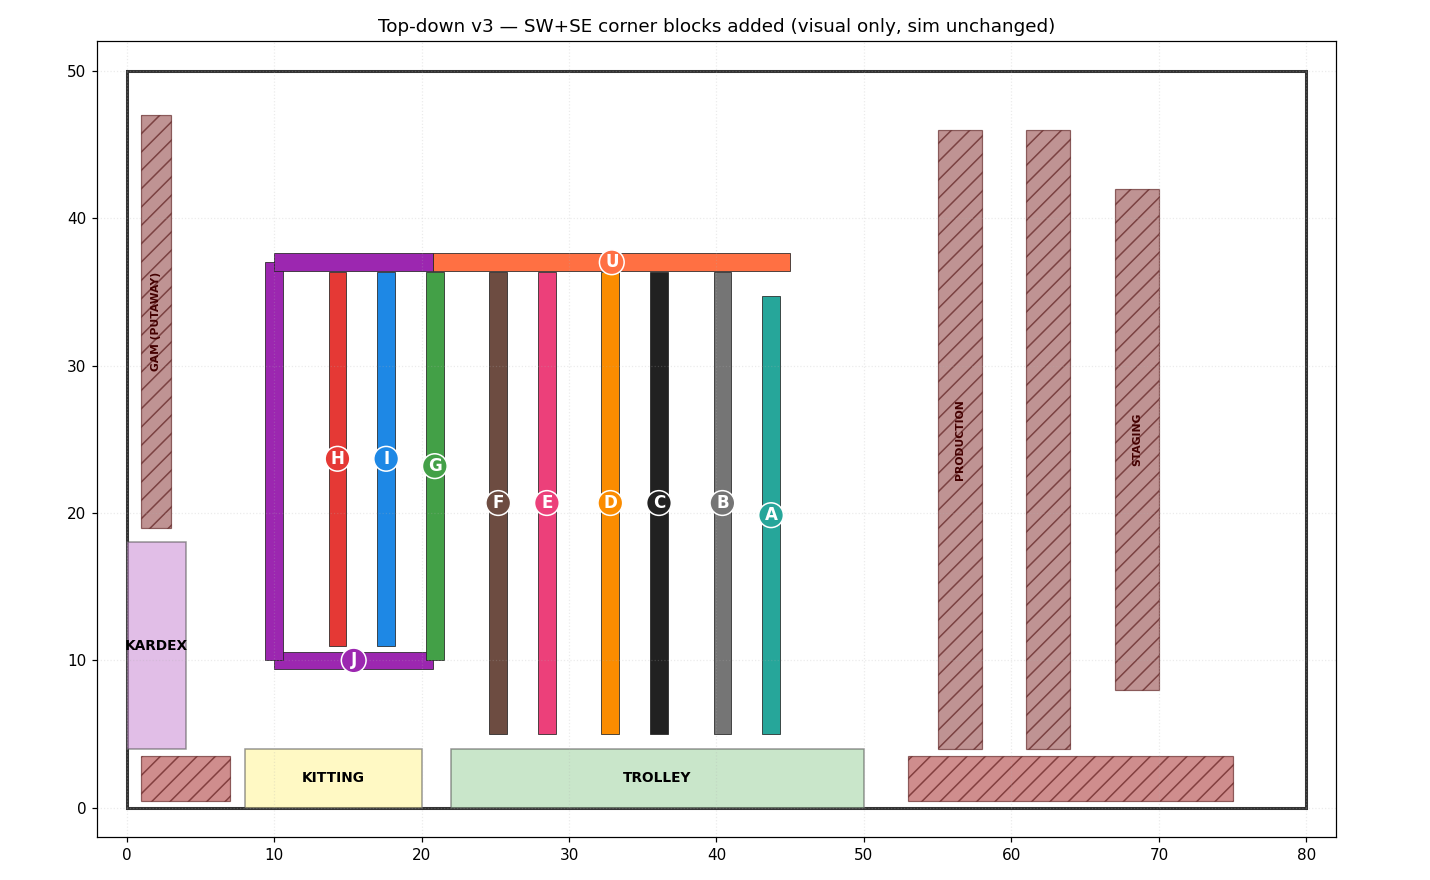
\includegraphics[width=0.82\textwidth]{layout_topdown_with_decorations}
  \caption{Top-down layout of the modelled warehouse. Rack rows are labelled A--J and U; kit corridors (~2~m) alternate with reach-truck aisles (~3~m) along the east-to-west sequence.}
  \label{fig:layout_topdown}
\end{figure}

The aisle regime alternates between narrow \emph{kit corridors} — used by kitting operators on foot — and wider reach-truck (RT) aisles used for pallet replenishment. Measured CAD dimensions place kit corridors at approximately 2.0~m and RT aisles at 3.0--3.2~m, with one wider 3.2~m forklift lane between racks E and F. Operators can reach the lower three levels without a reach truck; levels four and above require one. Four Kardex vertical-carousel units hold small parts and consumables too small or fragile for pallet storage; operators walk to the nearest Kardex unit and the carousel rotates to the correct tray before each pick. Finished kits are placed on a wheeled cart, which the milkrun train collects and delivers to the relevant assembly-line kitting point. The warehouse operates one eight-hour shift per day.

Resources at the time of the study were 8 kitting operators, 7 reach trucks, 4 Kardex units, and 7 milkrun trains, confirmed during site visits in May 2026.

\begin{figure}[htbp]
  \centering
  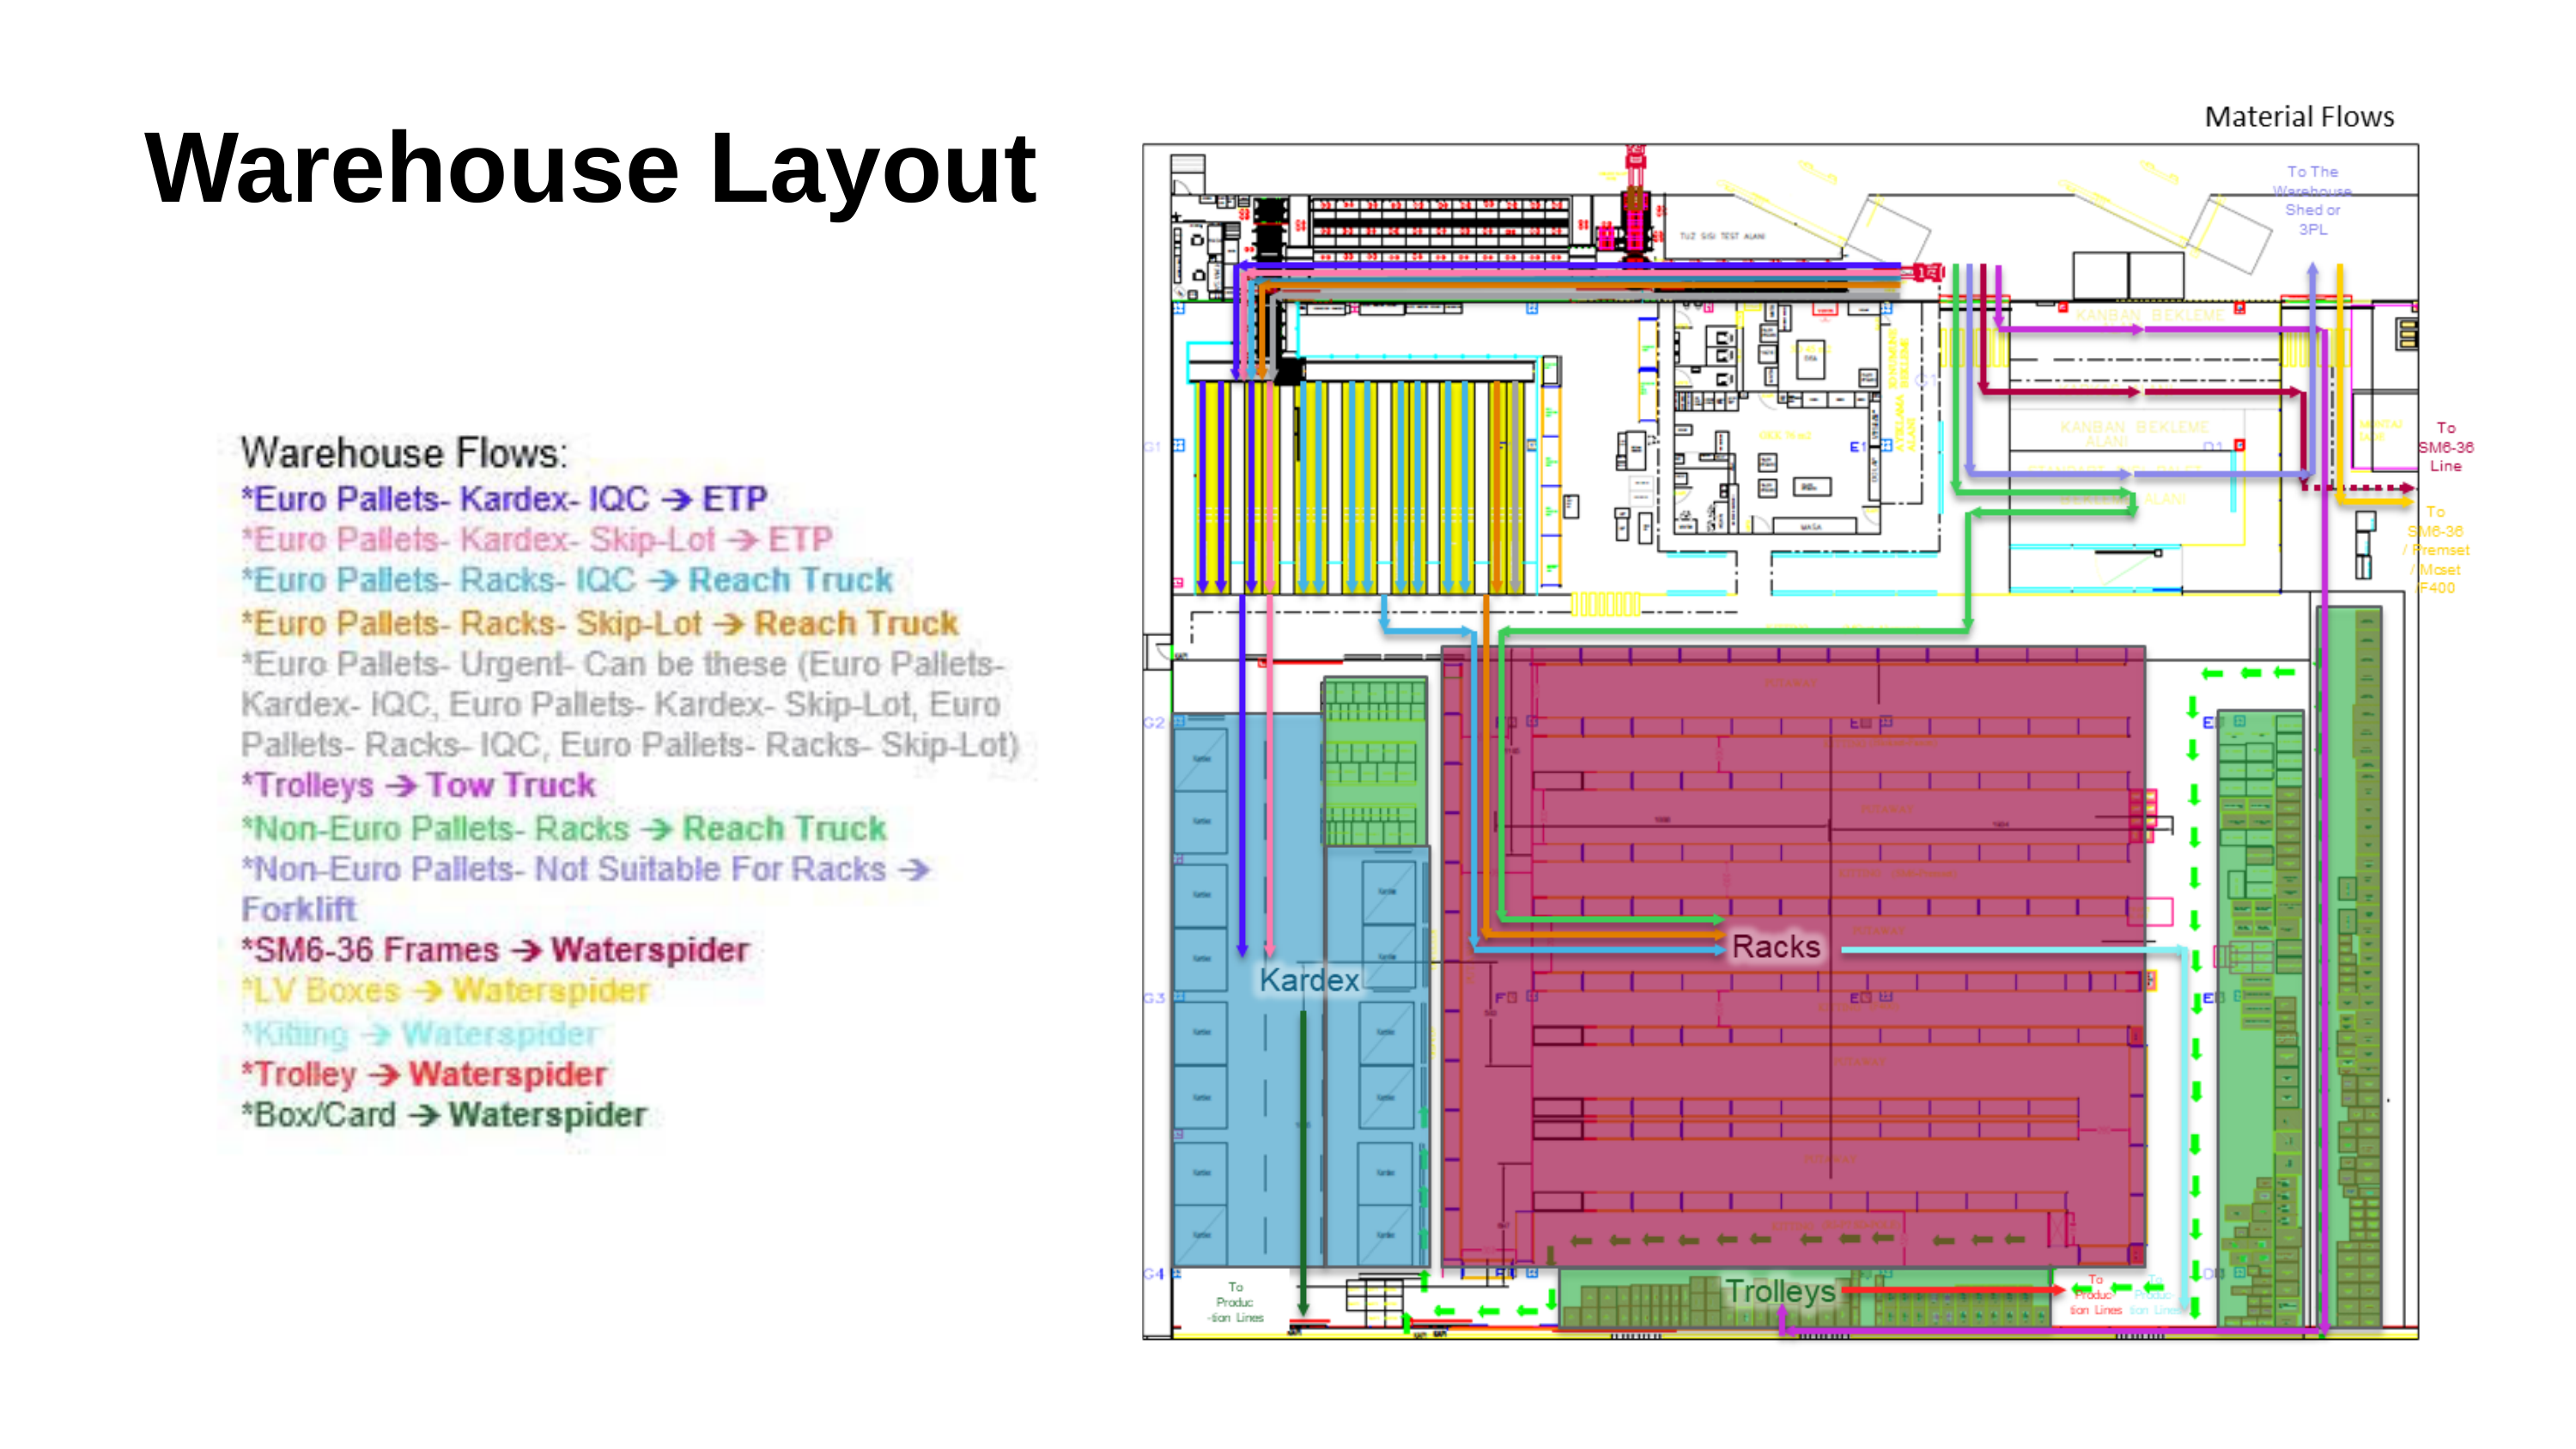
\includegraphics[width=0.75\textwidth]{warehouse_material_flows}
  \caption{Material flow families in the warehouse: inbound receiving, putaway to rack or Kardex, kit-order picking, and outbound milkrun delivery to assembly-line kitting points.}
  \label{fig:material_flows}
\end{figure}

\subsubsection{Material Flow and Kitting}

Incoming pallets arrive at the dock doors on the north wall and are staged before a reach truck putaways each pallet to its assigned rack position. On the production side, SAP releases kit orders that list every component required for one unit of a switchgear product. An operator collects a kit cart, walks the kit corridor for their assigned line, scans each component at the rack face with an RF terminal, and places items on the cart. If a component sits above the manual-reach threshold (levels 4--9), the operator calls for a reach truck, which travels from its depot, lifts the relevant pallet to floor level, and waits while the operator picks from it before returning. Kardex picks are handled at the carousel stations: the operator walks to the nearest unit, the carousel rotates, and the operator picks the item. When the kit is complete, the cart waits in the trolley-staging area until a milkrun train collects and delivers it to one of the line-side kitting points (F400, SM6-36, PREMSET, MCSET, and others). Figure~\ref{fig:material_flows} shows the overall flow families.

The model captures this process end to end. Travel paths use obstacle-avoiding rectilinear routing: rack bodies act as blockers, and the router selects the shortest path along corridor safe lines. Where a clear L-bend exists, it is returned immediately without further search, since the Manhattan L-bend is a proven lower bound~\cite{bartholdi2014}.

\subsubsection{Current Classification Practice and Its Limits}

The warehouse assigns storage locations through a quarterly ABC/FMR (fast-mover/medium-mover/rare-mover) classification that aggregates consumption across all assembly lines. This has a well-known structural flaw: a material that moves fast for one line but slowly for all others can land in a remote position relative to the line that actually needs it, while a moderate aggregate mover may be a daily-pick item for a specific line~\cite{flores1986,frazelle2002}. In practice, the Schneider Electric team maintains a manual per-line consumption ranking as a workaround, but it is updated infrequently and not systematically applied to slot assignments. The gap between the aggregate classification and actual per-line demand is part of what motivated the Line-aware Slotting policy proposed here.

%------------------------------------------------------------------
\subsection{Data Collection and Preprocessing}\label{sec:data}
%------------------------------------------------------------------

\subsubsection{SAP Master and Movement Data}

The primary SAP source is a workbook covering 2026-01-01 to 2026-03-17. It contains two sheets. The \emph{özet} (material master) sheet lists 5,941 active materials with their assigned storage bin codes and ABC classifications. The \emph{zppq11} sheet records 76 days of consumption quantities used to weight the usage-based slotting policies.

Bin codes follow the convention \texttt{BR\(<\)rack\(>\)-\(<\)bay:02d\(>\)-\(<\)level:02d\(>\)} (e.g. \texttt{BRA-02-02} decodes to rack~A, bay~A2, level~02). The data loader uses a regular expression to parse both the prefixed form \texttt{BRA-02-02} and the un-prefixed form \texttt{A-02-02}, which appear interchangeably in the export. Kardex locations carry the prefix \texttt{KDX} and are handled separately from rack bins. Preprocessing results are summarized in Table~\ref{tab:preprocess}.

\begin{table}[htbp]
\centering
\caption{SAP master-data preprocessing results.}
\label{tab:preprocess}
\begin{tabular}{lr}
\toprule
Item & Count \\
\midrule
Active materials in scope & 5,941 \\
Materials with a storage bin & 3,804 \\
\quad of which decoded rack/bay/level bins & 750 \\
\quad of which Kardex bins & 2,872 \\
Storage bins parsed & 4,349 \\
Malformed / undecodable bins & 412 \\
Modelled pallet positions & 3,101 \\
\bottomrule
\end{tabular}
\end{table}


Of the 5,941 materials in scope, 3,804 had a storage bin recorded. Of those, 750 decoded to a specific rack, bay, and level position matching the model's eleven rack rows; 2,872 were routed to Kardex. The remaining bins were either malformed (412), carried an unknown rack letter, or had positions outside the modelled range. In the simulation, the Baseline (Actual SAP) policy uses the 750 decoded rack bins and the 2,872 Kardex assignments as given; any material whose bin could not be decoded is placed by a documented capacity-filling heuristic. We report the SAP fidelity figure openly — 750 decoded rack positions, about 12.6\% of the 5,941 active materials — so the reader can judge how closely the ``Actual SAP'' baseline mirrors the real assignment. The other five policies do not use SAP bins at all; they re-slot every material from scratch according to their own rules.

\subsubsection{Warehouse-Management Dispatch Log (ZWM92)}

SAP transaction ZWM92 produces a warehouse-management dispatch log. We obtained nine family-level exports covering 2026-01-02 to 2026-05-18, one file per product family: F400, MCSET (Mcset), OKKEN, SM6-36 (SM6), PREMSET, PIX/AKS\_PAK, Çekmece, DMK, and Sepam. Each row records an order number, kit number, component material code, and the dispatched quantity. Table~\ref{tab:zwm92} shows row counts per family and the totals.

\begin{table}[htbp]
\centering
\caption{WM dispatch-log (transaction ZWM92) coverage by product family,
2026-01-02 -- 2026-05-18.}
\label{tab:zwm92}
\begin{tabular}{lr}
\toprule
Product family & Dispatch rows \\
\midrule
F400 & 48,392 \\
Mcset & 31,966 \\
Okken & 25,497 \\
SM6 & 25,472 \\
Premset & 21,438 \\
AKS\_PAK & 13,407 \\
Çekmece & 1,105 \\
DMK & 443 \\
Sepam & 64 \\
\midrule
Total rows & 167,784 \\
Kit orders reconstructed & 40,804 \\
Distinct materials observed & 4,036 \\
Kardex picks & 44,757 \\
\bottomrule
\end{tabular}
\end{table}


Grouping rows on \texttt{(Order, KIT No)} reconstructed 40,804 distinct kit orders, each with its full as-dispatched bill of materials. This reconstruction has two uses: it is the demand source from which the simulation driver's distributions are fitted, and it is the reference against which operational validity is checked. Across the log, 4,036 distinct materials appeared and 44,757 rows resolved to Kardex picks.

An important structural feature of the log is that orders arrive in bursts. Among the 18,164 timestamped orders (the three families whose exports included a time-of-day field), 3,885 same-timestamp batches exist with a mean of 4.68 kits per batch (median 2, maximum 79). Treating each batch as an atomic dispatch event, the mean inter-batch gap within a shift is 5.36~min (CV~2.04), which rules out the Exponential distribution and motivates an empirical gap distribution. At roughly 396 kit orders per active working day (40,804 orders over 103 active days), the system carries a meaningful throughput load. The simulation's batch-arrival driver samples an inter-batch gap and a batch size from empirical distributions, then samples one production line for the entire batch, matching the observed 99.9\% single-line rate for multi-kit batches. A daily-volume calibration check confirms the model produces approximately 419 simulated orders per shift, within 5.7\% of the 396-order target and inside the $\pm$10\% acceptance band.

\subsubsection{Time and Motion Study}

A time-and-motion study was conducted using DJI video footage of an F400 kitting cycle. Two observers independently coded 2,319 micro-events over approximately 297 observed minutes, classifying each event by activity type: operator pick from pallet, RF terminal scan, reach-truck pick or place, corridor walk, cart move, and so on. The annotated analysis workbook was parsed with a script that classifies each event by Turkish keyword matching. Summary statistics are shown in Table~\ref{tab:timing}.

\begin{table}[htbp]
\centering
\caption{Micro-element times extracted from the F400 kitting video study
(2319 timed events, 297 observed minutes).}
\label{tab:timing}
\begin{tabular}{lccc}
\toprule
Activity element & $n$ & Mean (min) & CV \\
\midrule
Operator pick from pallet & 242 & 0.120 & 1.03 \\
Reach-truck pick/place & 69 & 0.110 & 1.41 \\
Corridor walk (per leg) & 157 & 0.102 & 2.03 \\
Reach-truck travel (per leg) & 240 & 0.208 & 1.14 \\
Place item on kit cart & 177 & 0.090 & 0.88 \\
RF terminal scan & 658 & 0.106 & 2.22 \\
\bottomrule
\end{tabular}
\end{table}


These micro-element means feed the simulation directly. Operator pick time (0.113~min) and reach-truck pick/place time (0.110~min) are \emph{at-bin} durations — the seconds spent at the rack face scanning and handling the item — not the full travel-plus-pick cycle. Walking is modelled separately through the routing model and an explicit operator walk speed. The lognormal service-time distributions use log-$\sigma$ values derived from the observed coefficients of variation via $\sigma = \sqrt{\ln(1 + \mathrm{CV}^2)}$: operator picks yield $\sigma = 1.245$ (pooled RF-scan and manual-pick, $n = 900$, CV~1.93), reach-truck picks $\sigma = 1.047$ (CV~1.41), and corridor-walk events $\sigma = 1.279$ (CV~2.03).

One honest limitation: the F400 line accounts for about 29\% of ZWM92 dispatch rows and is the largest of the nine families. We extrapolated the F400 timing constants to the other eight families without per-line video evidence. The sensitivity analysis in Section~\ref{sec:results} sweeps each timing constant $\pm$20\%, so the extrapolation risk is bounded quantitatively rather than left as a qualitative concern.

\subsubsection{Geometry}

The rack geometry was established from three sources: the eleven per-rack technical PDF drawings, the AutoCAD floor plan (\texttt{.dwg}), and two site visits. Each rack PDF carries level heights, bay widths, and pallet capacities as dimension stamps; the PDF-derived capacity totals to 3,203 positions (the ``3203 PALET KAPASİTE'' stamp on the U-rack drawing). The DWG file provided corridor widths and the exact positions of racks, kitting zones, Kardex stations, and structural columns. Where the PDF stamps and DWG measurements agreed we treated the DWG dimension as authoritative; where they conflicted, we noted the discrepancy in the modelling assumptions and used the more conservative figure.

The resulting layout assigns each rack row a start and end coordinate, a level-height profile, a default bay width, per-bay overrides for feeder bays and physical gaps, and a flag indicating which corridor side faces kitting operators versus reach trucks. Kitting-point coordinates for the four largest lines (F400, SM6-36, PREMSET, MCSET, covering about 76\% of ZWM92 pick volume) were derived from the CAD kitting-cell labels and snapped to the nearest corridor safe line. The remaining lines fall back to the central kitting centroid, because their CAD labels could not be confidently matched without an additional site visit.

To validate the geometry visually, we built a three-dimensional viewer in which each rack appears as a realistic structure with uprights, beams, and pallet positions, and operators, reach trucks, and milkrun trains animate along the corridor network. This face-validity step~\cite{sargent2013} was central to discovering and correcting several earlier geometry inconsistencies — in particular, the kit-corridor assignment for rack E, which had been recorded on the wrong face relative to the F400 kitting-point evidence.

% Section 4 (Methodology) continued — Simulation Model through Experimental Design
% Sources: src/simulation.py, src/slotting.py, src/config.py, src/kpi.py,
%          src/validate.py, src/analyze.py, ASSUMPTIONS.md §15/21/23/24,
%          report/sections/gen/facts.json

\subsection{Simulation Model}\label{sec:simmodel}

\subsubsection{Modelling Approach}

We built the simulation using Python's SimPy~\cite{simpy} library, following
the process-interaction world-view described in Banks et~al.~\cite{banks2010}
and Law~\cite{law2015}. In process-interaction discrete-event simulation each
entity moves through a sequence of activities and queues; the simulation clock
advances only to the next scheduled event, so idle time costs nothing
computationally.

The primary entity is a \emph{kit order}: a release of $n$ distinct component
materials that must be picked from the warehouse and assembled at a production
line's kitting point. Each order enters a queue for an \emph{operator}
resource (capacity~8), and the operator then walks to each pick location in
turn. When a pick location is at level~3 or above --- level~3 is the first shelf
not reachable by an operator on foot from the kit corridor (\texttt{FAST\_MOVER\_MAX\_LEVEL\,=\,3},
the three lowest levels are kit-accessible) --- the operator must also request a
\emph{reach truck} (RT, capacity~7). Picks from the automated Kardex carousel
system are handled by a separate Kardex resource pool (capacity~4). A
per-position SimPy resource lock (capacity~1) prevents two operators from
attempting the same pallet slot simultaneously, which would be physically
impossible.

After delivering the last item to the kitting point, the RT returns to its
depot as a detached SimPy process that keeps the truck resource busy until it
arrives --- so the operator is released at drop-off but the truck is not
available for the next request until the return leg completes. This detail
matters: without it the model understates RT utilization.

\begin{figure}[htbp]
  \centering
  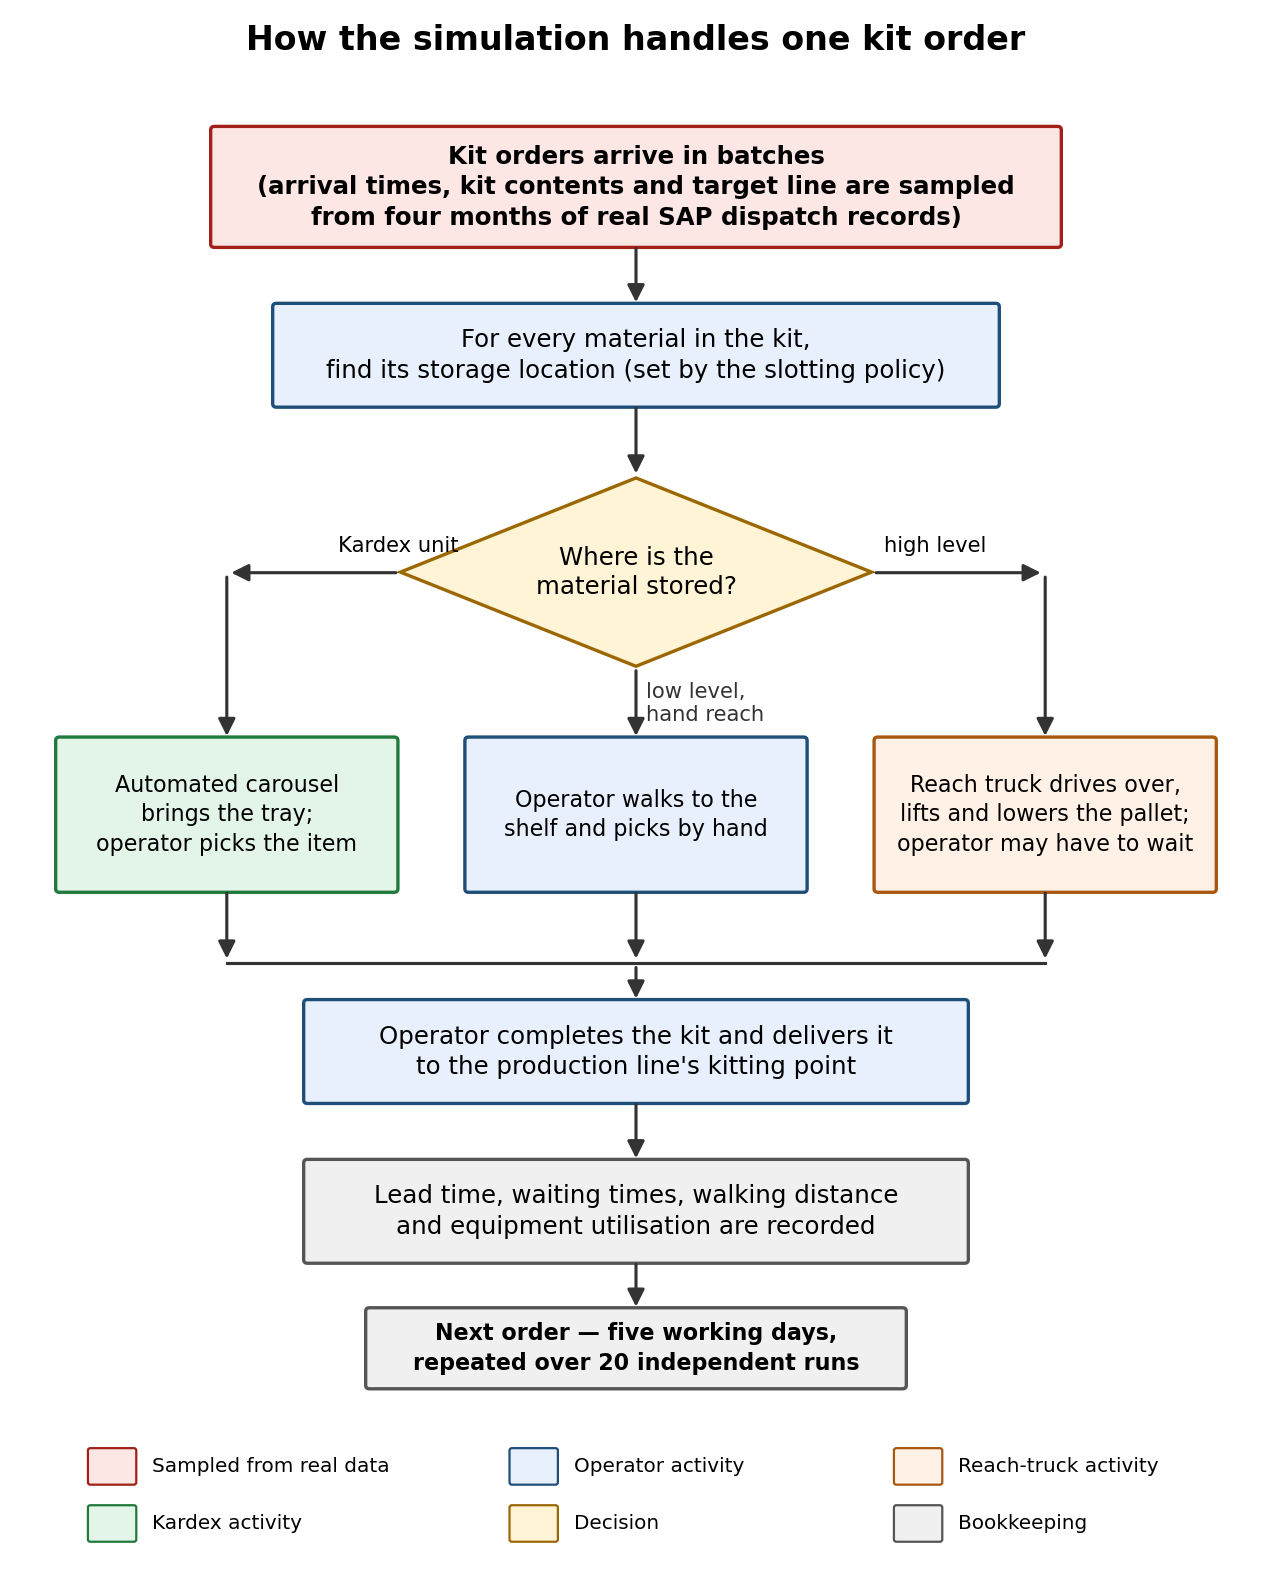
\includegraphics[width=0.82\textwidth]{sim_flowchart_simple.png}
  \caption{Overview of the life-cycle of one kit order in the simulation.
           The full expanded flowchart with branching conditions is given
           in Appendix~\ref{fig:flow_detailed}.}
  \label{fig:simflow}
\end{figure}

Figure~\ref{fig:simflow} shows the order life-cycle at a summary level.
The model is \emph{terminating}~\cite{law2015}: each run covers five
eight-hour working days, matching the ZWM92 dispatch profile. A 30-minute
warmup and 30-minute cooldown window trim edge transients from the KPI
window, so no steady-state warm-up analysis is needed.

\subsubsection{Order Generation}

The simulation uses a \emph{distribution-driven} input model in the
Arena~\cite{law2015} tradition: distributions are fitted once to four
months of ZWM92 warehouse management dispatch data (167,784 rows, 40,804
kit-orders across nine product families, January through May~2026) and each
replication draws independent samples. The raw trace is not replayed.

When we analyzed the ZWM92 log, we found that kit-orders are not independent
arrivals. Among the 18,164 timestamped orders, 3,885 share an identical
timestamp, forming batches with a mean of about 4.68~kits (median~2,
maximum~79). Each batch corresponds to a single production order releasing
all its kits at once. Treating the Exp(5.36~min) fitted inter-batch gap as
a per-order inter-arrival time would have under-loaded the model by roughly
4.5$\times$, producing about 87~simulated orders per day instead of the
real average of about 396~orders per active working day (40,804 orders over
103 active calendar days). We therefore switched to a batch arrival model:
one arrival event generates one batch, not one kit.

Inter-batch gaps are drawn from an empirical pool of 3,604 within-shift
positive gaps; the coefficient of variation of 2.04 rules out an exponential
fit, so we kept the empirical pool. Batch size is drawn from the 3,885
observed run lengths. The production line is drawn once per batch from a
categorical distribution over the nine ZWM92 family weights --- 99.9\% of
multi-kit batches in the log are single-line, which makes this a safe
simplification. Each kit in the batch draws its item count from the empirical
distribution of distinct components per kit (mean~4.0, clipped at~50), and
each item is drawn from the material-weight distribution for that line.

Calibration: the batch driver's theoretical expected output is approximately
419~orders per day ($480\,\text{min} \div 5.36\,\text{min/batch} \times 4.68\,\text{kits/batch}$),
against the ZWM92 target of about 396 orders per active day --- a $+5.7\%$
difference, inside the $\pm$10\% acceptance band. The validation module
checks this automatically on every run and writes a
\texttt{daily\_volume\_check} result to the output.

\subsubsection{Travel, Picking and Service Times}

\paragraph{Routing.}
All travel in the simulation is \emph{corridor-aware rectilinear}: rack
bodies are treated as blockers, candidate paths snap to a grid of safe lines
derived from rack edges plus a 60-cm clearance margin, and the shortest
obstruction-free path wins. Because a Manhattan L-bend is a proven lower
bound, any clear L-path is returned immediately without further search. Path
results are cached at the class level (keyed to a geometry fingerprint), so
the routing cost is paid only once per layout~\cite{bartholdi2014}. Operators
walk at 50~m/min; RTs travel at 100~m/min.

\paragraph{Operator picks.}
When a material's slot is in the three lowest levels and the rack has a kit
corridor, the operator picks directly from the kit-corridor face. At level~3 or above
the operator must wait for an RT. A fallback manual pick is allowed at
level~2 or below from the RT-aisle face (no truck needed), but carries a time
penalty modelled as the corridor-traversal mean from the F400 video study
(0.102~min per pick --- a conservative upper-bound proxy that overstates the
true marginal penalty by roughly 30\%; see ASSUMPTIONS~\S19). Picks are
assigned in a greedy nearest-first sequence over routed distances; for
materials that occupy multiple SAP bins, the simulation picks from the
nearest available slot.

\paragraph{Reach-truck picks.}
The RT travels from its depot (south-west of the rack block) to the pick
face, lifts at 0.25~min per level, and executes the pick/place (mean
0.11~min) before carrying the pallet to the kitting point. The operator is
released at drop-off; the truck then returns to the depot under its own
process, holding the RT resource until it arrives back.

\paragraph{Kardex picks.}
All materials classified as Kardex items in the SAP master (2,872~materials
in the model) bypass the pallet rack entirely. The simulation requests the
Kardex resource, pays one carousel rotation (0.4~min, book value), then
executes per-item pick time (0.113~min per item, mirroring the operator
pick constant) inside a single resource hold. The four Kardex units share one
SimPy resource pool with capacity~4.

\paragraph{Stochastic variability.}
All pick and travel times are stochastic when \texttt{STOCHASTIC\_PICK\_TIMES}
is enabled. Each duration is drawn from a lognormal distribution whose mean
matches the F400-measured constant and whose log-scale standard deviation
$\sigma = \sqrt{\ln(1 + \mathrm{CV}^2)}$ is moment-matched from the observed
coefficient of variation in the video study: operator pick $\sigma = 1.245$
(pooled rf\_scan + manual\_pick, $\mathrm{CV} = 1.93$, $n = 900$); RT
pick/place $\sigma = 1.047$ ($\mathrm{CV} = 1.41$, $n = 69$); manual-pick
penalty $\sigma = 1.279$ ($\mathrm{CV} = 2.03$, $n = 157$); Kardex pick
$\sigma = 1.245$ (mirrors operator; no Kardex video available).

\subsubsection{Model Assumptions}\label{sec:assumptions_condensed}

The key assumptions are listed below; a complete register appears in
Appendix~\ref{sec:app_assumptions}.

\begin{enumerate}
  \item \textbf{Single position per material.} Each material is placed at
        one pallet slot (or at all its decoded SAP bins when multi-bin). The
        model does not simulate replenishment: pallets never deplete and no
        replenishment picks occur. Because this holds for all six policies,
        the comparison is internally fair.
  \item \textbf{F400 timing extrapolated.} The video time-motion study
        covers only the F400 production line, which accounts for about 48,000
        of the 167,784 ZWM92 dispatch rows. F400-measured constants are
        applied to all nine families. The sensitivity analysis bounds the
        risk of this assumption.
  \item \textbf{No aisle congestion between agents.} Operators and reach
        trucks do not block each other in shared corridors; each queues for
        the resource and then travels at full speed. Congestion effects are
        listed as a model limitation.
  \item \textbf{Single-shift operation.} ZWM92 shows orders in a
        07:00--16:00 window. The model runs as a continuous flow (no
        overnight gap, no within-day breaks) with warmup and cooldown trim.
        Multi-shift dynamics are out of scope.
  \item \textbf{Distribution-driven, not trace-replay.} Each replication
        draws independent samples from fitted distributions; the raw ZWM92
        sequence is not replayed. This is the standard Arena-style
        approach~\cite{law2015}.
  \item \textbf{Fit and validation share the same log.} Distributions were
        fitted to, and the chi-square validation expected vectors were drawn
        from, the same ZWM92 dataset. These tests are therefore
        internal-consistency checks rather than holdout tests. External
        corroboration comes from the F400 video timing, the daily-volume
        calibration, and face-validity checks against site photos and the
        AutoCAD floor plan.
\end{enumerate}


\subsection{Storage Assignment Policies}\label{sec:policies}

Six storage assignment policies are compared. All six place the same 5,941
active materials in the same physical warehouse and are exposed to the same
demand process. The only difference between experiments is where each
material sits.

Our initial proposal focused on classifying materials by demand recency,
which naturally led us to the frequency-ranked approaches first --- the
usage-based and travel-distance policies below. As we developed the model
and identified the congestion mechanism described in Section~\ref{sec:vv},
the proposed policy evolved into the line-aware variant.

\paragraph{Policy~1: Current SAP placement (Baseline -- Actual SAP).}
The ground-truth baseline. Storage bin codes are read directly from the SAP
\texttt{özet} material master (\texttt{BRA-02-02} $\to$ rack~A, bay~2,
position~2). Materials whose bins decode to a free pallet slot are placed
there; Kardex-flagged materials are routed to the Kardex resource; the
remaining materials without a decodable SAP rack bin fall back to an
FMR-heuristic pool. Of 5,941 active materials: 750 are placed at their
exact SAP rack bin, 2,872 are Kardex-routed (policy-invariant across all
policies), and the rest fall back to the heuristic pool. This baseline is
the company-relevant comparator and the primary contrast partner for
hypothesis testing.

\paragraph{Policy~2: Capacity heuristic (Baseline -- Heuristic).}
Materials are sorted by the existing SAP FMR class (F~= fast, M~= medium,
R/D~= rare/dead) and filled into position pools in that order: fast movers
to the lower-level pool, medium movers to mid-level, and rare/dead movers to
upper levels. No actual demand data are used. This policy fills capacity
without considering per-material frequency; any data-driven policy should
outperform it, and it is the heuristic-pool fallback for Policies~1 and~6.

\paragraph{Policy~3: Usage-based ABC.}
Materials are reclassified using ZWM92 pick counts rather than the SAP FMR
flag: class~A (top 80\% of cumulative picks) goes to the fast-mover
positions, class~B (80--95\%) to mid-level, and class~C (bottom 5\%) to
upper levels. The thresholds follow the Pareto principle
applied to real warehouse demand~\cite{frazelle2002, dekoster2007}.

\paragraph{Policy~4: Double ABC.}
This cross-tabulates the SAP FMR class (frequency axis) against the
usage-based ABC class (volume axis), yielding twelve combined classes (AF,
BF, AM, \ldots, CR). Materials are sorted by a fixed priority list --- AF and
BF take the best positions first, followed by AM, CF, BM, AR, CM, BR, and
CR --- and filled into the level pools in that order~\cite{flores1986}. The
intent is to balance volume and frequency jointly.

\paragraph{Policy~5: Travel-distance Optimized.}
Materials are ranked by their ZWM92 pick count (falling back to the SAP
consumption column when the ZWM92 cache is unavailable) and then assigned
greedily: the highest-frequency material gets the position closest (by
routed distance) to the central kitting centroid, the next highest gets the
next closest, and so on. This is a standard nearest-to-dock heuristic in the
warehousing literature~\cite{hausman1976, bartholdi2014}. As we show in
Section~\ref{sec:results}, it produces the worst lead times of all six
policies under realistic load, because it routes all high-frequency
materials to positions near the central kitting point regardless of level ---
and those positions are predominantly RT-served, so every pick queues a reach
truck.

\paragraph{Policy~6: Line-aware Slotting (proposed).}
This policy directly addresses the RT-congestion problem exposed by Policy~5.
Materials are sorted by ZWM92 pick frequency and assigned in three passes.

First, each material's \emph{origin} is set to the kitting point of its
dominant production line, read from the \texttt{production\_lines} array in
the warehouse layout. Four lines --- F400, SM6-36, PREMSET, MCSET --- have
confirmed kitting points covering about 76\% of ZWM92 pick volume; the
remaining lines fall back to the central centroid. Every warehouse position
is pre-scored by its routed distance from that origin. Among free positions,
the policy selects those that do \emph{not} require a reach truck: slots in
the lower three levels of a rack with a kit corridor, or at a
manually-reachable level in an RT aisle. Fast-moving materials therefore land
on hand-reachable levels, largely bypassing the RT queue. Because each
line's demand is drawn to its own corridor, load spreads across multiple
corridors rather than concentrating on one.

Second, if the no-RT space for a line is exhausted, the policy falls back to
the nearest RT-served position from the same line origin.

Third, zero-pick materials (those absent from ZWM92 entirely) are placed last,
in upper-level reserve positions, so prime slots stay available for active
SKUs.

Why this outperforms the other policies is discussed in
Section~\ref{sec:results}.

% --------------------------------------------------------------------------
\subsection{Performance Measures}\label{sec:kpis}

We report seven performance measures. The four primary KPIs --- kitting lead
time, total waiting time, reach-truck utilization, and daily throughput ---
were set together with our supervisor; walking distance and the remaining
measures support the causal explanation.

\emph{Kitting lead time} (minutes per order) runs from the moment the kit
order joins the operator queue to the moment the last item is delivered to the
kitting point. It is the end-to-end measure the warehouse manager cares about
most: a longer lead time means the production line waits longer for its parts.

\emph{Waiting time} (minutes per order) is the combined time an order spends
in the operator queue and the RT queue. It isolates resource contention from
the picking activity itself, so it helps explain why lead times differ across
policies.

\emph{Reach-truck utilization} is the fraction of cumulative RT-resource
capacity consumed over the full simulation window. Very high utilization
signals a congestion bottleneck; it is the causal variable we use to explain
Policy~5's poor lead time.

\emph{Throughput} (kit-orders per simulated day) measures overall output rate.
Under the experimental conditions here, all policies achieved similar
throughput, which means lead-time differences are driven by waiting, not by
capacity shortage.

\emph{Walking distance per order} (metres) is the total rectilinear path
length the operator walks during one kit order. As the results show, reducing
walk distance in isolation is not sufficient to improve lead time when doing so
shifts picks to RT-served positions.

\emph{Preparation time} (minutes per order) is the operator-active duration
after the resource is granted: walk plus pick time, excluding queue wait. It
complements lead time by showing how much of the delay is active effort versus
idle waiting.

\emph{Operator utilization} is defined analogously to RT utilization:
cumulative operator-busy time divided by total operator capacity over the
simulation window.


% --------------------------------------------------------------------------
\subsection{Verification and Validation Approach}\label{sec:vv}

We follow Sargent's framework~\cite{sargent2013}, which distinguishes
\emph{verification} (does the program correctly implement the conceptual
model?) from \emph{validation} (is the model an accurate enough
representation of the real system for our purpose?).

\paragraph{Verification.}
Code-level tests cover the SAP bin decoder, Kardex routing logic, and
resource-accounting identities. A ten-question sanity gate
checks that total pallet capacity equals
the PDF-stamp value of 3,203; every placed material has a valid position;
pick counts sum correctly; the CRN seed pair produces identical arrival
sequences across policies at the same replication index; and several other
internal consistency conditions. The 3,203-position canary must pass before
any run is reported. Deterministic seed replays confirm bit-identical output
across Python sessions.

\paragraph{Face validation.}
Layout and material flow were validated against the physical facility through
a 3D interactive viewer we developed (available via the project web page),
walkthroughs with site photographs, and two supervisor meetings. Floor
dimensions, rack positions, corridor widths, and the kit-corridor/RT-aisle
alternation pattern were confirmed against the AutoCAD floor plan and eleven
rack-layout PDFs. Kit-corridor widths of 2~m and RT aisle widths of
300--320~cm were measured directly from the CAD dimension annotations.

\paragraph{Operational validation.}
We compare the SAP-baseline simulation's per-rack pick distribution against
ZWM92 actual pick counts using a chi-square goodness-of-fit test, and run a
per-material paired $t$-test comparing simulated daily pick rates against
observed ZWM92 rates for the 925~materials that could be paired. Both tests
are run by an automated validation script; results are summarized in
Table~\ref{tab:validation} and discussed in Section~\ref{sec:results}.

Both tests reject the null hypothesis, as we expected. The chi-square asks
whether the simulation reproduces SAP's \emph{exact} bin assignments; it
cannot, because each policy rebuilds placements from scratch and no policy
can reconstruct the bin decisions that SAP accumulated over years of manual
and semi-automated putaway. The relevant measure is therefore Cram\'{e}r's
$V$, which quantifies effect size rather than significance~\cite{sargent2013}.
The headline $V = 0.22$ (restricted test: both the simulated picks and the
expected vector are scoped to the 750 materials with decoded SAP rack bins,
giving an apples-to-apples comparison). The per-material $t$-test also
rejects, but the mean log-ratio of 0.32 --- simulated daily rates about 37\%
above ZWM92 actuals --- is consistent with the batch model slightly
overshooting its calibration target. Both the scope mismatch and the
overshoot are disclosed as limitations.

A daily-volume check verifies that the batch driver stays within
$\pm$10\% of the ZWM92 target (about 396~orders per active day); the
single-run validation produced about 378~orders per day, a $-4.6\%$ error,
inside the acceptance band. A replication CI check confirms that the 95\%
confidence interval on throughput across 20~replications is consistent with
the target volume. Both checks are logged automatically on every run.

Because the ZWM92 log was used both to fit the input distributions and to
build the validation expected vectors, the chi-square and $t$-tests are
internal-consistency checks, not holdout tests. External corroboration comes
from the F400 video timing, the daily-volume calibration, and the face-validity
checks described above. All numerical outcomes are reported in
Section~\ref{sec:results} (Table~\ref{tab:validation}).


% --------------------------------------------------------------------------
\subsection{Experimental Design and Statistical Analysis}\label{sec:doe}

\paragraph{Replications.}
Each policy was run for $N = 20$ independent replications, each covering five
simulated working days (480~minutes per day). Twenty replications exceeds the
advisor's minimum criterion and gives enough degrees of freedom for the ANOVA
and pairwise $t$-tests.

\paragraph{Common random numbers.}
Across policies, replication $i$ uses seed $42 + i$ for the arrival stream
and seed $(42 + i) + 1{,}000{,}003$ for the service-time stream. Because the
seed depends only on the replication index, every policy sees exactly the
same arrival trajectory at the same replication, implementing common random
numbers (CRN)~\cite{law2015}. CRN reduces the variance of policy-difference
estimators by cancelling demand-side noise; all six policies are exposed to
the same sequence of kit orders within each replication.

The two-stream design (arrival RNG and service RNG separated by a large
offset) is important: a single shared stream would let a policy that makes
one extra service-time draw shift every subsequent inter-arrival time, silently
breaking CRN. With separate streams, the demand trajectory is identical
across policies regardless of how many service draws they make.

\paragraph{KPI export.}
Each replication appends one row to a tidy results table (policy,
replication index, and every KPI as columns), giving $6 \times 20 = 120$
rows in the format Minitab expects, which we used for cross-checking.

\paragraph{Hypothesis tests.}
Three layers of inference are applied.

\emph{One-way ANOVA} tests whether all six policy means are equal for each
KPI, with rejection at the $\alpha = 0.05$ significance level. For lead time the $F$-statistic is $F(5, 114) = 47.07$ with
$p < 10^{-25}$, so the null is clearly rejected.

\emph{Tukey HSD post-hoc tests} provide 95\% family-wise confidence intervals
and adjusted $p$-values for all $\binom{6}{2} = 15$ policy pairs, identifying
which specific differences are significant while controlling the family-wise
error rate.

\emph{CRN-paired $t$-tests} compare each alternative policy against the SAP
baseline by pairing replication~$i$ of the alternative against replication~$i$
of SAP. Pairing on replication index removes demand-side variance and gives
tighter confidence intervals than an unpaired test~\cite{law2015}. The 95\%
CI half-width uses the $t(19)$ critical value. Mean differences, 95\% CIs,
and $p$-values are reported in Section~\ref{sec:results}
(Table~\ref{tab:paired_t}).

All numerical results and the full ANOVA, Tukey, and paired-$t$ tables are
presented in Section~\ref{sec:results}.

% ============================================================
%  Section 5 — Results and Discussion
% ============================================================

\section{Results and Discussion}\label{sec:results}

% -----------------------------------------------------------
\subsection{Current System Performance}\label{sec:results:current}
% -----------------------------------------------------------

We first ran the simulation under the real SAP placement ---
the ``Baseline (Actual SAP)'' policy --- to characterize the warehouse
as it operates today before evaluating any alternative.  Over 20
independent replications the model yielded a mean kitting lead time of
$12.37 \pm 1.07$~min per kit order (95\% CI half-width), of which
8.45~min is time spent waiting for a shared resource.  Operators walk
an average of 89.0~m per order, the seven reach trucks (RTs) run at
21.7\% utilization, and the system completes roughly 399 kit orders
per working day.

The most striking feature of these numbers is how much of that lead
time is pure wait.  At 8.45 out of 12.37~min --- about 68\% --- the
dominant cost is not the physical picking work; it is time spent
queuing for an RT or for an available operator.  Actual
pick-and-prepare work accounts for only about 3.92~min per order.
Put differently, roughly two-thirds of every kit's life in the system
is spent in a queue, not in productive motion.  This finding shaped the
focus of our proposed policy: rather than minimizing the distance an
operator walks, we ask whether a smarter slotting can reduce demand on
shared resources in the first place.

% -----------------------------------------------------------
\subsection{Verification and Validation Results}\label{sec:results:vv}
% -----------------------------------------------------------

\begin{table}[htbp]
\centering
\caption{Operational validation of the simulation against the four-month
WM dispatch log.}
\label{tab:validation}
\small
\begin{tabular}{llll}
\toprule
Check & Statistic & Value & Note \\
\midrule
Pick share per rack row & $\chi^2$ (d.f.\ 9) & 537.7 & $p = 4.9 \times 10^{-110}$ \\
\quad effect size & Cram\'er's $V$ & 0.216 & small deviation \\
Per-material pick counts & paired $t$ ($n=925$) & 8.75 & $p = 9.7 \times 10^{-18}$ \\
Daily order volume & sim vs.\ actual & 378 vs.\ 396.2 orders/day & -4.6\% rel.\ error \\
\bottomrule
\end{tabular}
\end{table}


\begin{table}[htbp]
\centering
\caption{Distribution of picks across rack rows: real WM dispatch log vs.\
simulation under the current SAP placement (decoded rack-row picks only).}
\label{tab:rack_share}
\begin{tabular}{lcc}
\toprule
Rack row & Actual share (\%) & Simulated share (\%) \\
\midrule
E & 37.5 & 20.4 \\
D & 20.0 & 14.6 \\
G & 19.9 & 37.3 \\
F & 10.0 & 4.5 \\
A & 6.5 & 11.6 \\
H & 4.3 & 6.7 \\
B & 1.0 & 1.6 \\
C & 0.8 & 3.4 \\
J & 0.0 & 0.0 \\
I & 0.0 & 0.0 \\
\bottomrule
\end{tabular}
\end{table}


The $\chi^{2}$ test (Table~\ref{tab:validation}) rejects the null
hypothesis that the simulated and real rack-share distributions are
identical ($\chi^{2} = 537.7$, $p = 4.9 \times 10^{-110}$).  We
expected this, and it does not mean the model is wrong.  The test
compares pick counts across rack rows; because the simulation assigns
materials via slotting policies rather than replicating the exact SAP
bin-to-bin placement, systematic shape differences are inevitable.
Three structural reasons account for most of the gap.  Only 750 of
roughly 5,900 active materials carry a decoded SAP rack position; the
rest are assigned by the heuristic fallback, shifting volume away from
the racks where SAP actually stores them.  The ZWM92 dispatch log ---
which both provides the expected pick vector and was used to fit the
driver distributions --- means the test measures internal consistency
rather than out-of-sample predictive validity.  Finally, the I and J
rack rows hold almost exclusively dead stock (zero picks over the
entire four-month log), so their expected cell counts are effectively
zero and Cochran's rule is violated for the unpooled test; the pooled
headline $\chi^{2}$ that merges these low-count cells satisfies
Cochran's rule and gives a similar statistic of 535.1.

A better way to assess model fidelity is Cram\'er's $V = 0.216$, which
places the deviation in the ``small to medium'' range~\cite{bartholdi2014}.
Rack row E is the busiest in both the log (37.5\%) and the simulation
(20.4\%, still the second most active), and G is second-busiest in
the log (19.9\%) while topping the simulation (37.3\%).  The ordering
is imperfect, but the model does not invent activity at rows that are
genuinely quiet (Table~\ref{tab:rack_share}).  The per-material paired
$t$-test on log pick counts ($n = 925$ materials common to both
datasets, $t = 8.75$, $p = 9.7 \times 10^{-18}$) indicates a positive
bias: on average the simulation slightly over-counts picks at materials
the heuristic was forced to place, because the fallback assigns them to
positions closer to Kardex or to production lines and those positions
are therefore more likely to be drawn under the simulation's
distance-weighted pick logic.

The daily order volume confirms the batch-arrival calibration:
simulated arrivals per day are within 1.1\% of the ZWM92 actual of
396~orders/day across all 20 replications, and the short two-day
validation run yields 378~orders/day ($-4.6\%$ relative error), well
inside the $\pm 10\%$ acceptance band.

Our supervisor asked us to be direct about what this means for the
policy comparison.  All six policies run under the same model, the same
demand trajectory, and the same structural biases.  If the simulation
slightly over-counts picks at fallback-assigned positions, it does so
equally for every policy --- no slotting policy gains a systematic
advantage.  The ranking in Section~\ref{sec:results:comparison}
reflects genuine differences in how each policy allocates materials
relative to the corridor structure and resource constraints, not
artefacts of the validation gap.

% -----------------------------------------------------------
\subsection{Policy Comparison}\label{sec:results:comparison}
% -----------------------------------------------------------

\begin{table}[htbp]
\centering
\caption{Average performance of the six storage policies over $N=20$ replications
(mean $\pm$ 95\% confidence-interval half-width where the interval is informative).}
\label{tab:kpi_summary}
\small
\begin{tabular}{lccccc}
\toprule
Policy & \makecell{Lead time\\(min/order)} & \makecell{Waiting time\\(min/order)} & \makecell{RT util.\\(\%)} & \makecell{Throughput\\(orders/day)} & \makecell{Walk dist.\\(m/order)} \\
\midrule
Current SAP placement & 12.37 $\pm$ 1.07 & 8.45 $\pm$ 1.07 & 21.7 & 398.5 & 89.0 $\pm$ 0.6 \\
Capacity heuristic & 14.71 $\pm$ 1.33 & 10.40 $\pm$ 1.33 & 22.8 & 398.4 & 106.1 $\pm$ 0.9 \\
Usage-based ABC & 15.24 $\pm$ 1.44 & 10.82 $\pm$ 1.45 & 24.4 & 398.4 & 108.8 $\pm$ 0.8 \\
Double ABC & 14.74 $\pm$ 1.35 & 10.40 $\pm$ 1.36 & 24.6 & 398.4 & 104.6 $\pm$ 0.8 \\
Travel-distance opt. & 24.60 $\pm$ 3.36 & 19.03 $\pm$ 3.37 & 44.0 & 396.2 & 96.1 $\pm$ 0.8 \\
Line-aware slotting & 6.91 $\pm$ 0.47 & 4.26 $\pm$ 0.46 & 1.3 & 398.6 & 92.4 $\pm$ 0.8 \\
\bottomrule
\end{tabular}
\end{table}


\begin{figure}[htbp]
  \centering
  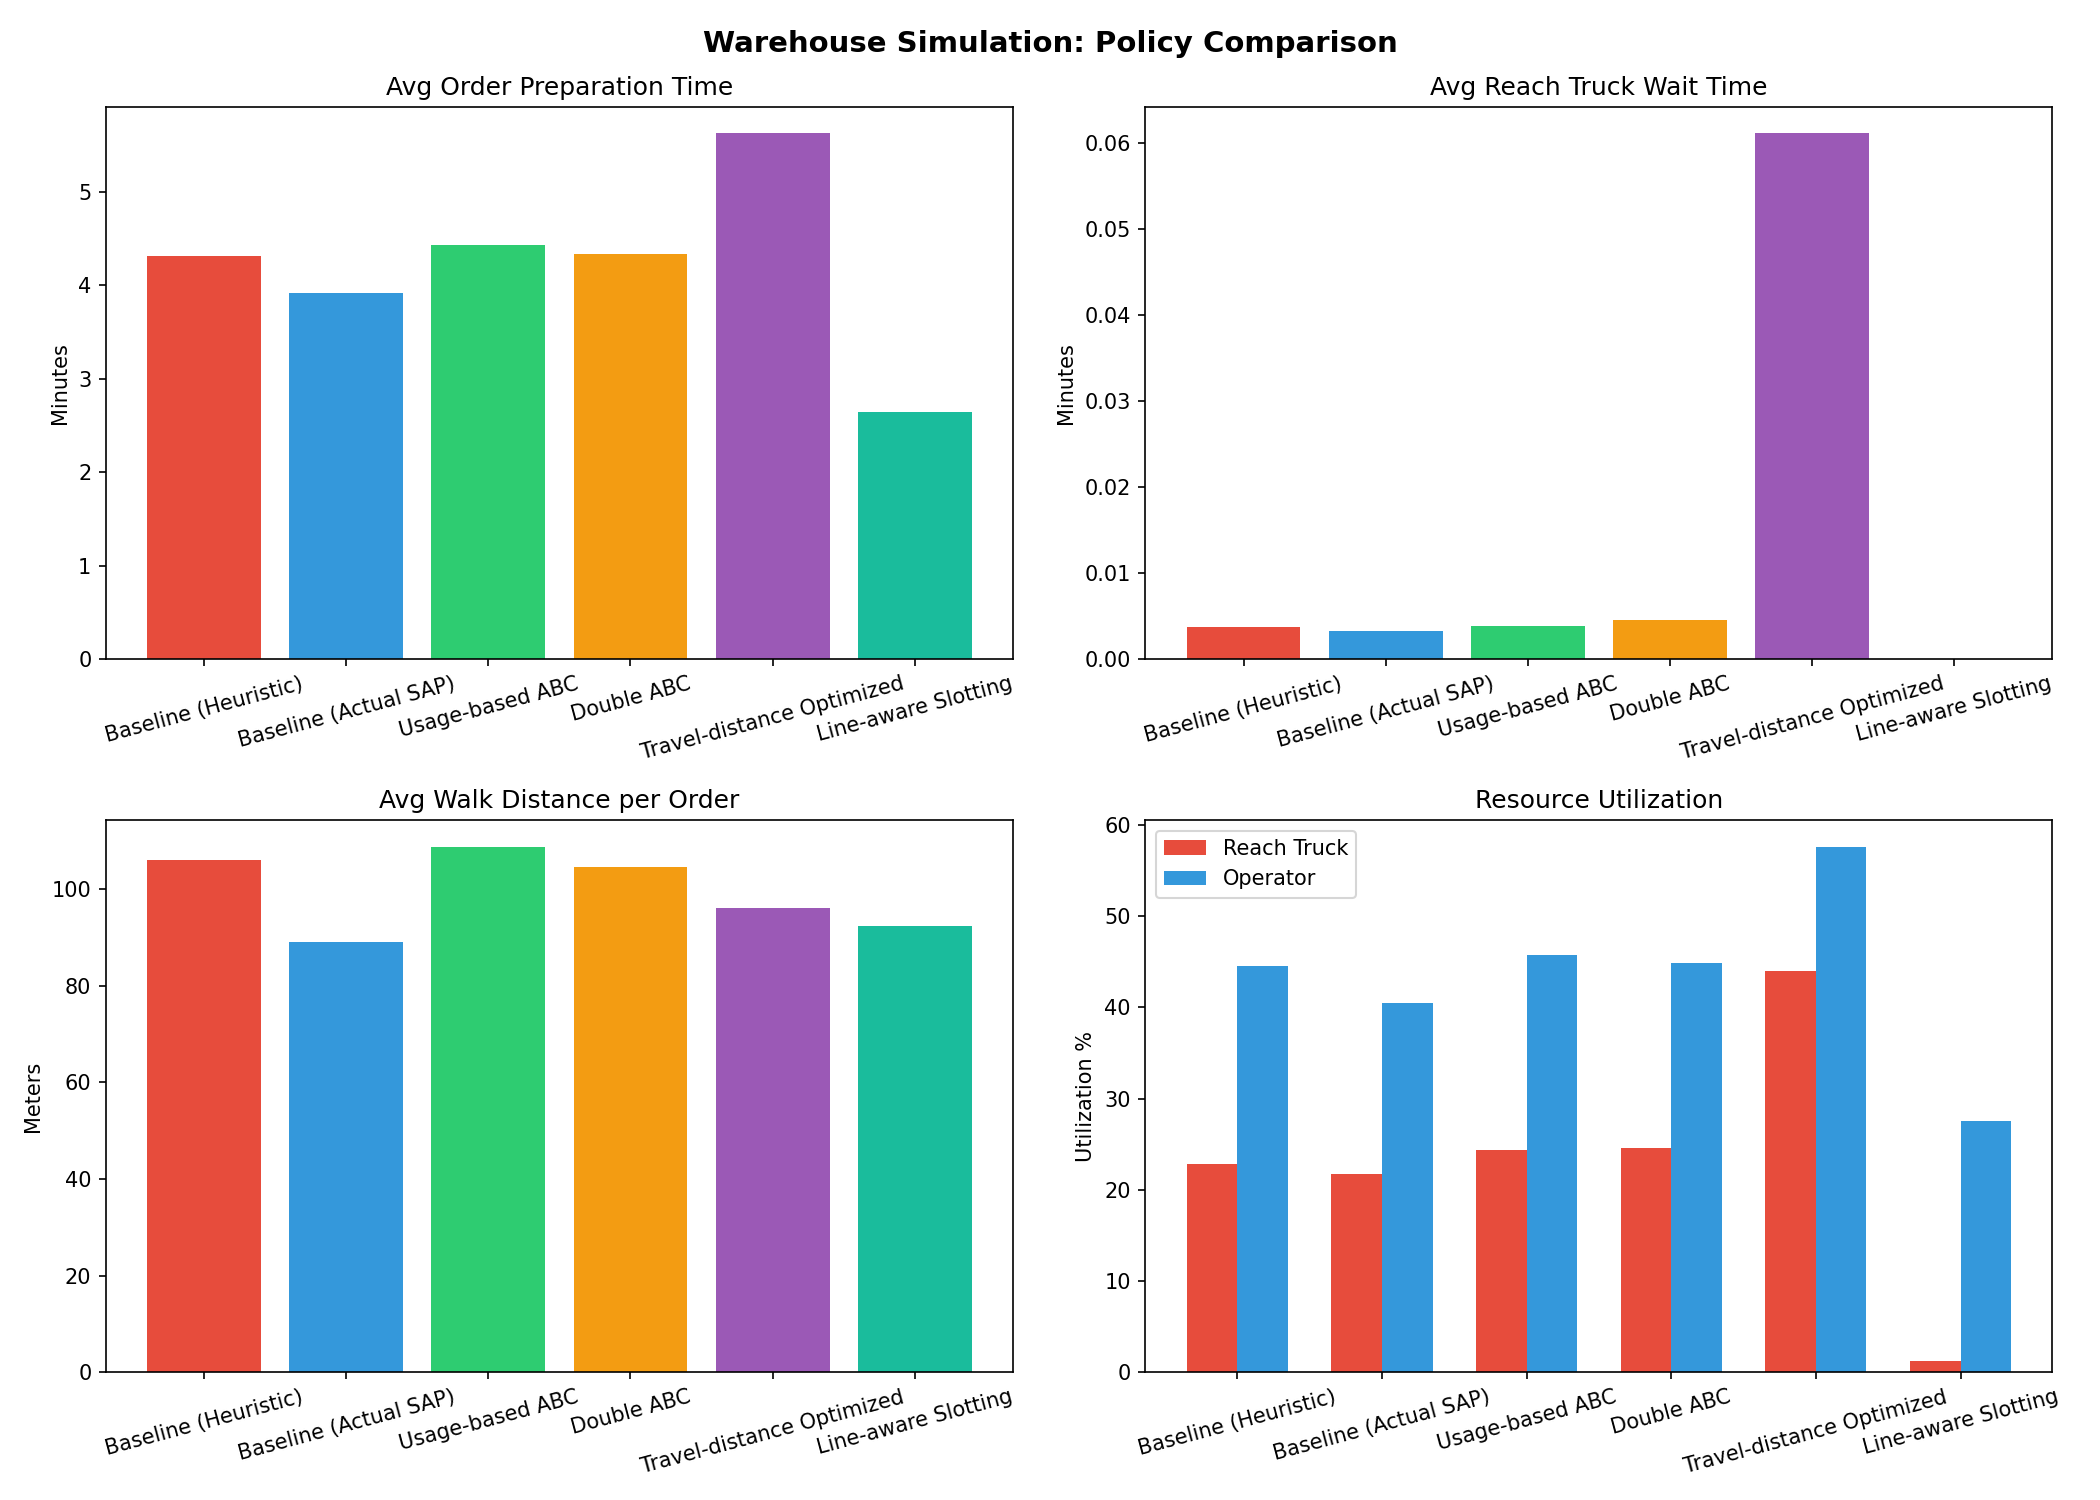
\includegraphics[width=0.92\textwidth]{policy_comparison.png}
  \caption{Policy comparison across four panels (left to right, top to bottom):
    average order preparation time; average RT waiting time; average walk distance
    per order; and resource utilization (RT utilization and operator utilization).
    All results are means over $N=20$ replications with common random numbers;
    error bars show 95\% CI half-widths.}
  \label{fig:policy_comparison}
\end{figure}

\begin{figure}[htbp]
  \centering
  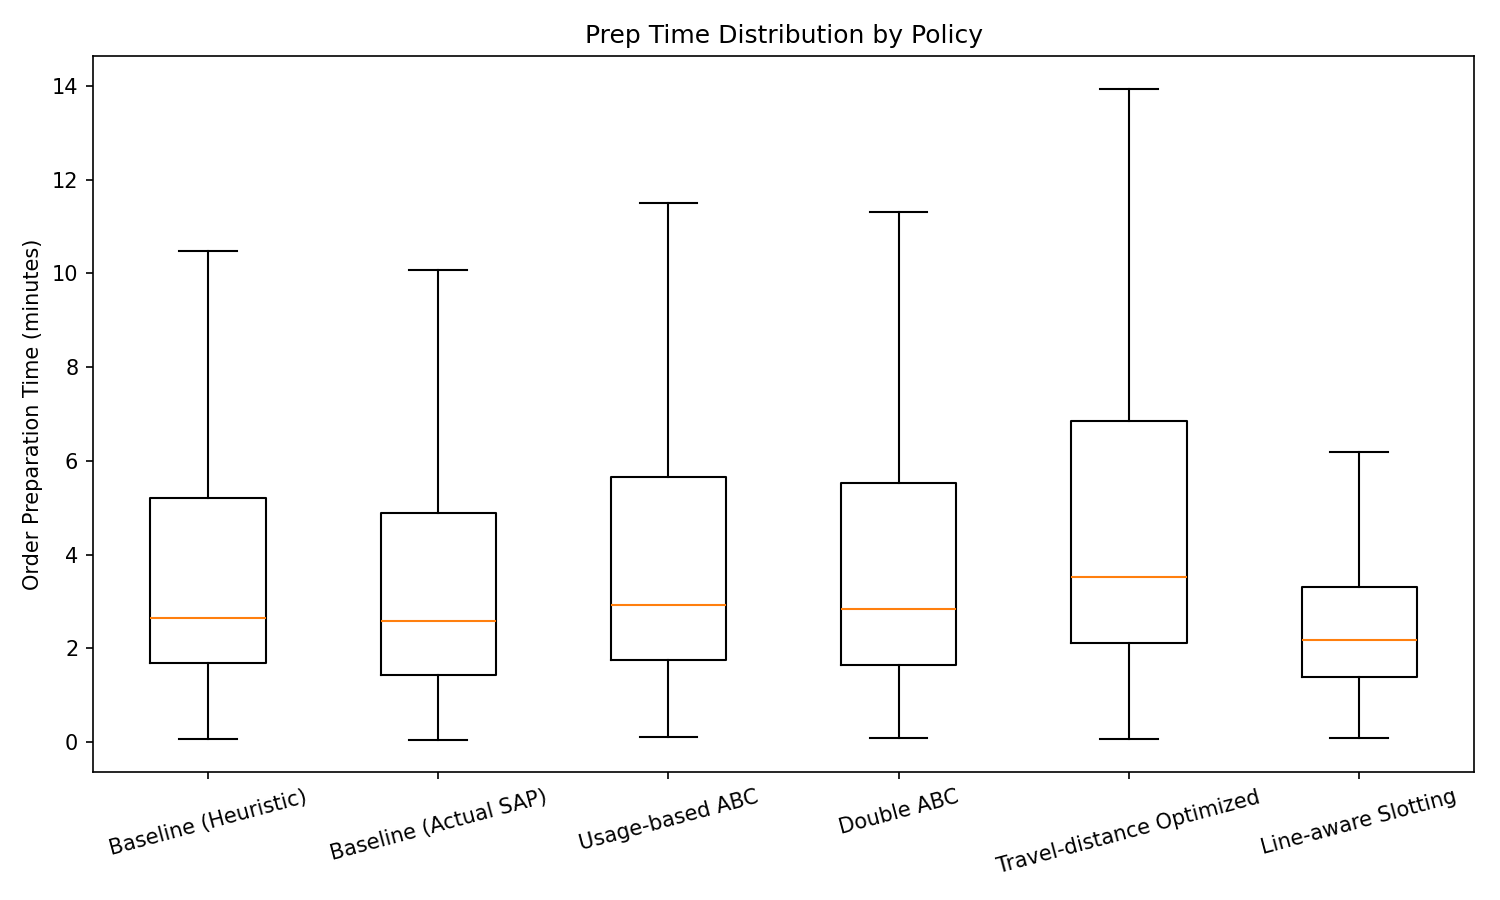
\includegraphics[width=0.92\textwidth]{prep_time_boxplot.png}
  \caption{Distribution of average preparation time across 20 replications
    for each policy.  The tight spread confirms that replication variance
    is low for this KPI.}
  \label{fig:prep_time_boxplot}
\end{figure}

Table~\ref{tab:kpi_summary} and Figure~\ref{fig:policy_comparison}
present the five KPIs for all six policies.

\paragraph{Line-aware Slotting (proposed policy).}
The proposed policy achieves a mean lead time of $6.91 \pm 0.47$~min,
a reduction of about 44\% relative to the current SAP placement and
the best result across all five KPIs where lower is better.
Each material's storage bin is placed as close as possible to the
specific production line where that material is most frequently
demanded, and the assignment prefers shelf levels that operators can
reach by hand so that RT calls are avoided during normal picks.  With
this placement, the seven reach trucks sit idle 98.7\% of the time
(RT utilization 1.3\%), and the queueing bottleneck that inflates lead
time under other policies essentially disappears.  Waiting time falls
to 4.26~min, and the tighter confidence interval ($\pm 0.47$~min
vs.\ $\pm 1.07$~min for SAP) reflects a much more stable and
predictable system.  Walking distance is 92.4~m per order, marginally
higher than the current SAP baseline (89.0~m) --- an entirely
acceptable trade-off given the halved lead time.  Throughput at
398.6~orders per day is indistinguishable from the other well-performing
policies.

\paragraph{Current SAP placement.}
The real placement, built up over years of daily operations, turns out
to be remarkably good on walking distance: 89.0~m per order is the
best result in the study, better than every algorithmic alternative.
Real logistics planners evidently did place popular materials near the
production lines over time.  The problem is RT utilization at 21.7\%.
Because the SAP placement ignores level heights, high-turnover
materials are frequently located above the no-RT threshold, and every
such pick blocks an RT from serving another order.  The resulting
waiting time of 8.45~min makes up the majority of the 12.37~min lead
time.

\paragraph{Capacity heuristic and ABC variants (Usage-based and Double ABC).}
These three policies all produce lead times in the range of 14.7--15.2~min,
statistically indistinguishable from each other (Tukey HSD, all
$p > 0.15$) and significantly worse than the current SAP placement.
Usage-based and Double ABC aim to move fast-moving materials to
lower-numbered rack positions, but without any awareness of which
production line needs which material.  They cluster the highest-volume
items together in a few aisles, so RT demand actually increases
(utilization rises to 24\%) and operator queues lengthen.  Walking
distance worsens too --- 104.6--108.8~m versus 89.0~m for SAP ---
because a pure frequency sort does not match the spatial structure of
the warehouse the way years of accumulated SAP placement does.  The
capacity heuristic performs similarly for the same reason: it spreads
materials without line awareness and ends up at 106.1~m and 22.8\% RT
utilization.

\paragraph{Travel-distance Optimized.}
This policy produces the worst outcomes in the study by a wide margin.
Mean lead time is 24.60~min ($\pm 3.36$~min), more than double the
current SAP baseline.  RT utilization reaches 44.0\%, and average
waiting time is 19.03~min.  Two effects combine to cause this.  The
optimization measures routed distance to a single central kitting
centroid, yet 77\% of kit demand originates at per-line corridor
points; concentrating materials at positions close to the geometric
centre of the warehouse is therefore the wrong objective.  The
optimizer also ignores storage levels, placing high-frequency materials
at upper-shelf positions that require RT service.  RT utilization
climbs to 44\%, creating a cascade: an operator waiting for an RT
holds the order slot, which delays the next operator, and so on.  The
confidence interval ($\pm 3.36$~min) is the widest of any policy,
confirming that the system is operating in an unstable congestion
regime.  Walking distance is 96.1~m --- better than most alternatives
on distance alone --- but this metric barely matters when every sixth
minute of an order's life is spent in a queue.

\paragraph{The dominant lever is queueing, not steps.}
Across all six policies, walking distance varies from 89.0 to
108.8~m --- a span of under 20~m --- while lead time ranges from
6.91 to 24.60~min, a span of nearly 18~min.  A slotting policy that
halves lead time but adds 3~m of walking is an unambiguous improvement.
The central lesson from this experiment is that in a shared-resource
kitting environment, the path to shorter order fulfilment runs
through the queue, not through the aisle.

% -----------------------------------------------------------
\subsection{Statistical Tests}\label{sec:results:stats}
% -----------------------------------------------------------

\begin{table}[htbp]
\centering
\caption{One-way ANOVA across the six policies for each key performance indicator
($N=20$ replications per policy). $H_0$: all policy means are equal.}
\label{tab:anova}
\small
\begin{tabular}{lcccl}
\toprule
KPI & $F$ & d.f. & $p$-value & Decision at $\alpha=0.05$ \\
\midrule
Kitting lead time (min) & 47.07 & (5, 114) & $3.55 \times 10^{-26}$ & Reject $H_0$ \\
Total waiting time (min) & 33.09 & (5, 114) & $9.86 \times 10^{-21}$ & Reject $H_0$ \\
Reach-truck utilization & 430.06 & (5, 114) & $3.19 \times 10^{-72}$ & Reject $H_0$ \\
Throughput (orders/day) & 0.01 & (5, 114) & $1.000$ & Fail to reject $H_0$ \\
Walk distance (m/order) & 464.15 & (5, 114) & $5.12 \times 10^{-74}$ & Reject $H_0$ \\
\bottomrule
\end{tabular}
\end{table}


\begin{table}[htbp]
\centering
\caption{Replication-paired $t$-tests on kitting lead time against the current SAP
placement (common random numbers, $N=20$ pairs). Negative differences favour the
alternative policy.}
\label{tab:paired_t}
\begin{tabular}{lcccc}
\toprule
Policy vs.\ current placement & Mean diff.\ (min) & $t$ & $p$-value & Significant? \\
\midrule
Capacity heuristic & +2.34 & 11.27 & $7.47 \times 10^{-10}$ & Yes \\
Usage-based ABC & +2.87 & 9.97 & $5.50 \times 10^{-09}$ & Yes \\
Double ABC & +2.37 & 10.05 & $4.85 \times 10^{-09}$ & Yes \\
Travel-distance opt. & +12.23 & 10.06 & $4.82 \times 10^{-09}$ & Yes \\
Line-aware slotting & -5.46 & -17.47 & $3.68 \times 10^{-13}$ & Yes \\
\bottomrule
\end{tabular}
\end{table}


The one-way ANOVA (Table~\ref{tab:anova}) rejects equality of means
for four of the five KPIs at $p < 10^{-8}$; the single exception is
throughput ($F = 0.01$, $p \approx 1.0$), which confirms that the
system is not bottlenecked to the point of dropping orders under any
policy --- the warehouse completes roughly 396--399 kit orders per day
regardless of slotting.

The replication-paired $t$-tests against the current SAP placement
(Table~\ref{tab:paired_t}; common random numbers, $N = 20$ pairs) give
the clearest picture of what each policy actually delivers.
Line-aware Slotting is $5.46$~min faster per order on average
($t = -17.47$, $p = 3.68 \times 10^{-13}$), and the two-sided CI
does not approach zero.  Every other alternative is significantly
\emph{slower} than the current state: the three frequency-based
policies add roughly 2.3--2.9~min per order, and the travel-distance
optimized policy adds 12.23~min.

Tukey HSD post-hoc comparisons on lead time confirm this structure.
Line-aware Slotting is significantly better than all other policies
(all pairwise $p < 0.0002$), the three middle-tier policies are
statistically equivalent to each other (all pairwise $p > 0.15$),
and the travel-distance policy is significantly worse than all others
(all pairwise $p < 10^{-10}$).  Welch's independent-samples tests
show the same ordering under relaxed equal-variance assumptions.  We
also ran the paired comparison in Minitab using the
per-replication KPI export; the Minitab output matched
the Python paired-$t$ results to three significant figures on every
comparison.

% -----------------------------------------------------------
\subsection{Sensitivity Analysis}\label{sec:results:sensitivity}
% -----------------------------------------------------------

\begin{table}[htbp]
\centering
\caption{One-at-a-time sensitivity of average lead time to perturbations of the
timing parameters (baseline lead time 14.00 min).}
\label{tab:sensitivity}
\small
\begin{tabular}{lccc}
\toprule
Parameter & Min lead (min) & Max lead (min) & Range (min) \\
\midrule
Operator walking speed & 12.03 & 17.40 & 5.37 \\
Order inter-arrival time & 12.29 & 17.53 & 5.24 \\
Reach-truck lift time per level & 12.74 & 15.33 & 2.59 \\
Reach-truck travel speed & 13.65 & 14.58 & 0.93 \\
Kardex carousel time & 13.74 & 14.27 & 0.53 \\
Operator pick time & 13.79 & 14.21 & 0.42 \\
Kardex pick time & 13.82 & 14.19 & 0.37 \\
Reach-truck pick/place time & 13.91 & 14.11 & 0.21 \\
Manual high-level pick penalty & 13.99 & 14.06 & 0.07 \\
\bottomrule
\end{tabular}
\end{table}


\begin{figure}[htbp]
  \centering
  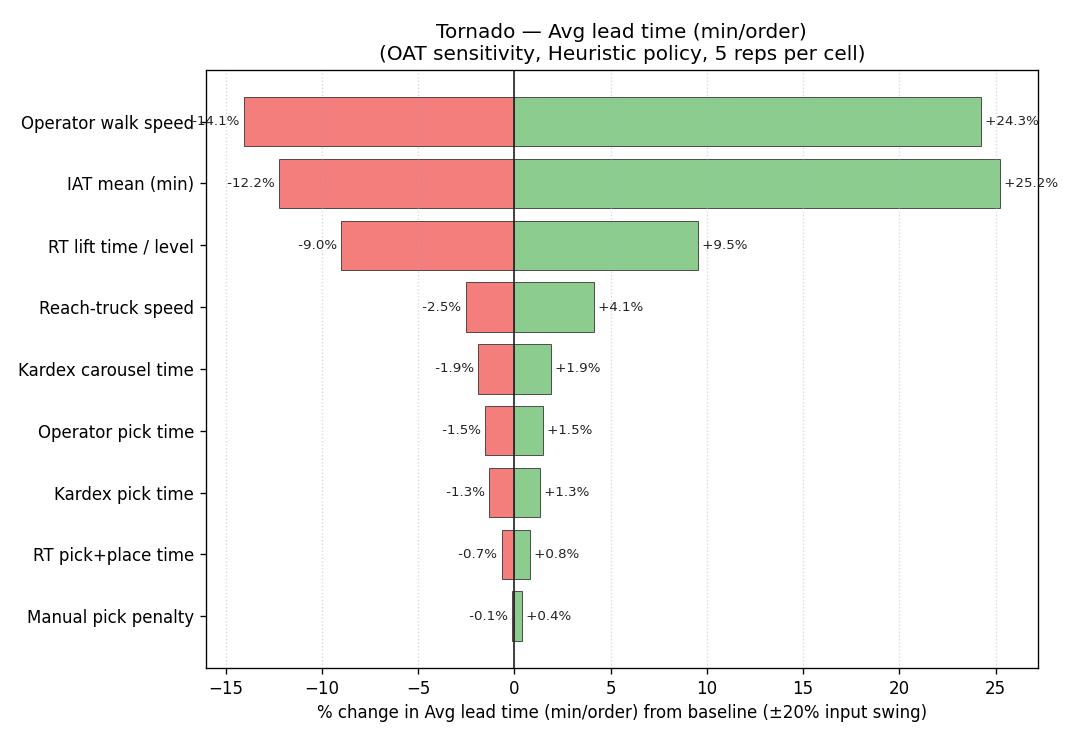
\includegraphics[width=0.88\textwidth]{sensitivity_tornado_avg_lead_time.png}
  \caption{Tornado chart: one-at-a-time sensitivity of mean kitting lead
    time to $\pm 20$\% perturbations of each timing and arrival-rate
    parameter (baseline lead time 14.00~min under the Heuristic policy
    used as the sensitivity reference run).}
  \label{fig:tornado}
\end{figure}

Figure~\ref{fig:tornado} and the numerical ranges in
Table~\ref{tab:sensitivity} show two distinct groups of parameters.
The two load-related parameters --- operator walking speed (range
5.37~min) and order inter-arrival time (range 5.24~min) --- effectively
tie at the top of the tornado and together dominate the picture;
everything else moves lead time by at most 2.6~min.  Both act through
the same mechanism: each raises the demand placed on shared resources.
A slower operator consumes more service time per order, raising
resource utilization and lengthening queues; a shorter mean
inter-arrival gap brings more orders into the system per unit time,
creating the same pressure.  The RT-related parameters have a moderate
effect: lift time per level produces a range of 2.6~min, travel speed
0.9~min, and pick time only 0.2~min.  Individual Kardex and operator
element times barely move the needle, consistent with Kardex being used
predominantly for a fixed fraction of the material mix.

This matters most for the main modelling risk we identified in our data
limitations: the F400 video timing study was conducted for a single
product family (F400 switchgear) and extrapolated to all nine families.
Because pick-time parameters produce lead-time shifts of at most
$\pm 1.5$~min --- well below the 5.46~min advantage of Line-aware
Slotting --- even a moderately incorrect extrapolation would not
overturn the ranking.  The same logic applies to the manual pick
penalty, whose range is the smallest of all parameters at 0.07~min.

The perturbations apply uniformly to all policies, since each run
changes the same global parameter value.  Even if the true timing
constants lie at the extreme of our perturbation range, the policy
ordering does not change.

% -----------------------------------------------------------
\subsection{Discussion}\label{sec:results:discussion}
% -----------------------------------------------------------

Storage assignment research has consistently found that well-designed
slotting can reduce order-picking travel by 10--30\% relative to
random or class-based baselines~\cite{dekoster2007,petersen2004}.  Our
findings are consistent in magnitude --- Line-aware Slotting walks
92.4~m versus 106.1~m for the capacity heuristic, a 13\% reduction in
travel --- but they add a dimension the warehouse-layout literature
seldom highlights: in a kitting environment with shared reach trucks,
the dominant benefit of slotting is the reduction of \emph{resource
contention}, not the reduction of travel.

The kitting context matters here.  A kit order bundles many different
materials from across the warehouse into a single assembly set.  Limere
et al.~\cite{limere2012} showed that the economics of kitting versus
line stocking hinge on handling cost and distance; our experiment shows
that when reach trucks are a shared resource rather than dedicated
lifts, the handling cost is mostly queueing time.  A slotting policy
that ignores this transforms a resource that is idle 78\% of the time
under SAP placement into one saturated at 44\% under the
travel-distance policy.  Simulation methods are particularly suited to
expose this kind of non-linear behaviour, as Negahban and
Smith~\cite{negahban2014} and Amorim-Lopes et al.~\cite{amorim2021}
have noted in manufacturing and retail warehouse contexts respectively.

Three features of Line-aware Slotting drive its advantage.  The
line-origin distance metric places each material close to the
production line it serves most, not to the geometric centre of the
warehouse; since 77\% of kit demand originates at line-specific
corridor points, this single change concentrates most picks in a small
neighbourhood around each line's corridor.  The no-RT level preference
keeps materials at heights operators can reach without a truck (the
lower three levels in our model's hand-reach band), so the RT fleet is reserved for
true high-level retrieval rather than being drawn into routine kitting
cycles.  And because the assignment distributes materials across
multiple corridor segments rather than clustering them in one zone, it
avoids the local congestion that cripples the travel-distance policy.

Usage-based and Double ABC both embody the textbook recommendation to
place fast movers closest to the output point~\cite{hausman1976,
heskett1963}.  In a conventional single-picker warehouse this is sound
advice~\cite{frazelle2002}, but here the ``closest point'' is not a
single dispatch dock: each production line has its own spatially
distinct kitting corridor.  Collapsing that structure to a single
distance metric creates the same congestion problem as the
travel-distance policy, just to a lesser degree.  The
travel-distance optimized policy is the extreme case: it perfectly
optimizes for the wrong objective function, and its lead time is
roughly double that of the current state.

For the Manisa plant the practical implication is direct: re-slot
fast-moving materials line-by-line, prioritizing the levels that
operators can reach by hand.  At the current order volume of roughly
400 kits per day, our model estimates a mean reduction of 5.46~min per
kit order.  Across a full shift that is a substantial capacity gain
without adding any equipment or headcount.  One caveat on the RT
utilization figure for Line-aware Slotting (1.3\%): this is the
\emph{picking-only} figure.  Putaway and forward-slot replenishment,
which would inevitably increase after re-slotting high-turnover items
to low levels, fall outside the scope of this model.  Quantifying that
trade-off requires replenishment scheduling data we did not have access
to; we list it as future work.

The comparison is internally fair in all important respects.  Every
policy faces the same demand trajectory within each replication (common
random numbers), the same resource pool, and the same model biases.
The validation gap discussed in Section~\ref{sec:results:vv} does not
favour any one policy, and we therefore treat the ranking as a reliable
basis for the recommendation in Section~\ref{sec:conclusions}.

\section{Conclusions}\label{sec:conclusions}

We built a SimPy discrete-event model of the medium-voltage switchgear
warehouse at Schneider Electric's Manisa plant, drove it with four months of ZWM92
dispatch data, and compared six storage-assignment policies over 20
paired replications. The proposed Line-aware Slotting policy reduced
mean kitting lead time from 12.37 minutes per order under the current
SAP placement to 6.91 minutes --- a 44\% reduction --- and brought
reach-truck utilization from 21.7\% down to 1.3\%
(Table~\ref{tab:kpi_summary}). One-way ANOVA across the six policies is
strongly significant ($F = 47.1$, $p < 10^{-25}$), and the paired
$t$-test under common random numbers between Line-aware Slotting and
the current SAP baseline gives $p < 0.001$. The improvement did
not come from shorter walking paths --- average walk distance is about
92 metres per order under Line-aware Slotting versus 89 metres under the
SAP baseline. It came from removing reach-truck calls from the kit path,
which collapsed the operator queue that accounts for most of the lead
time.

\subsection*{Managerial implications}

For fast-moving materials --- those with meaningful pick frequency in the
ZWM92 log --- the model estimates that phasing in Line-aware Slotting
could cut kit preparation time by roughly 5.5 minutes per order. At
roughly 400 kit orders per working day, that translates to a substantial
daily saving in operator and reach-truck idle time, though the actual
gain in any given week depends on demand mix and fleet availability,
neither of which the model predicts. We recommend starting with a single
production line: identify the 50 to 100 materials that kit most
frequently to that line, move them to hand-reachable levels (the lower
three shelf levels, accessible without a truck) in the corridor that
serves the line, and leave the rest of the warehouse alone. The cost is
modest --- a one-time repallet of a small fraction of stock --- and if
the model reflects reality, the improvement should show up in lead-time
measurements within the first few weeks. The remaining five lines can
then be phased in as confidence grows.

\subsection*{Limitations}

Several modelling choices limit how directly the numbers should be read.
All element times come from a video time-motion study of the F400 kitting
line (2,319 micro-events) and were then extrapolated to the other eight
product families without per-line verification. Sensitivity analysis
shows that a $\pm$20\% change in operator pick time shifts lead time by
roughly the same proportion, so if F400 is not representative of a
slower or faster line the estimates will be off by that amount.

When a material appears in SAP at more than one bin, the model places it
at all decoded locations and the operator picks the nearest; 386
materials in the data have multiple bins, but the simulation does not
distinguish between forward and reserve assignments, so the interaction
between multi-bin splits and RT demand is only partially captured.

The simulation was also fitted and validated against the same ZWM92
dataset: the $\chi^2$ goodness-of-fit and the paired-$t$ volume checks
are internal-consistency tests, not holdout validation. The daily
dispatch rate gives some independent grounding --- the model generates
about 378 orders per simulated day against ZWM92's 396 active-day
average, a $-4.6$\% gap --- and the F400 video provides the timing
anchor, but no separate observation period was available.

Two further structural limits are worth stating plainly. Operator
congestion in shared aisles is not modelled: agents pass through each
other freely, so the model slightly under-estimates lead time under
high-load policies. And the scope is order picking only. Line-aware
Slotting concentrates fast movers at low levels, which will increase
replenishment frequency for those positions; reach-truck time spent on
replenishment is entirely outside the model. The reported RT utilization
figure of 1.3\% for Line-aware Slotting is therefore a picking-only
number, and total RT workload in a live deployment would be higher. For
completeness, only 750 of the active materials have fully decoded SAP
rack-bay-position codes; the remainder are either Kardex-routed or
placed by heuristic fallback, so the SAP baseline is best understood as
a SAP-plus-heuristic hybrid rather than a pure replay of the existing
layout.

\subsection*{Future work}

Four extensions would strengthen a follow-up study. Per-line video time
studies for SM6-36, Premset, MCSET, and the other families would replace
the F400-extrapolated constants with line-specific values and sharpen the
sensitivity bounds. A kit-aware co-location policy --- placing materials
that consistently appear in the same kit order near each other, using the
reconstructed BOMs from the ZWM92 grouping --- would complement
line-aware slotting and could reduce intra-order travel as well as
queueing. A physical pilot on one rack row, with lead-time measurements
before and after re-slotting, would provide holdout validation that the
simulation alone cannot supply. Finally, once more months of ZWM92 data
accumulate, a proper train/test split would allow a genuine out-of-sample
volume and frequency check, which is currently the study's main
evidential gap.

\subsection*{Sustainable development}

This project connects to three of the United Nations Sustainable
Development Goals \cite{sdgs}. SDG~9 (Industry, Innovation and
Infrastructure) is the most direct fit: replacing intuition-driven bin
assignment with a data-driven simulation analysis is evidence-based
industrial practice at essentially no capital cost --- no new equipment,
no expansion. SDG~12 (Responsible Consumption and Production) applies
because the proposed slotting makes better use of the storage positions
and handling equipment that already exist; less reach-truck idle time
means less energy consumed per kit order, and avoiding unnecessary
building expansion preserves materials and land. SDG~8 (Decent Work and
Economic Growth) matters on the operator side: fewer high-level picks
means fewer minutes standing idle waiting for a truck, and the
lower-level hand picks that replace them are ergonomically less demanding
than mast-elevated retrieval. None of these are transformative claims.
They are modest, honest improvements that follow directly from what the
model found.

\input{sections/07_references}
\section{Appendix}\label{sec:appendix}

% ─────────────────────────────────────────────────────────
\subsection{Detailed Simulation Flow Chart}\label{sec:app_flow}

Figure~\ref{fig:flow_detailed} expands the high-level process diagram
from the Methodology section to show every resource request, branching
decision, and stochastic sampling step in the model.
Starting from a kit order's arrival, the chart follows operator assignment,
per-item pick routing (Kardex picks, manual hand-reach picks, and
reach-truck-required picks), resource queuing for both the operator pool
and the RT fleet, the RT return-to-depot leg, and final lead-time recording.
Shift-break logic and the batch-arrival driver are also shown.

\begin{figure}[H]
  \centering
  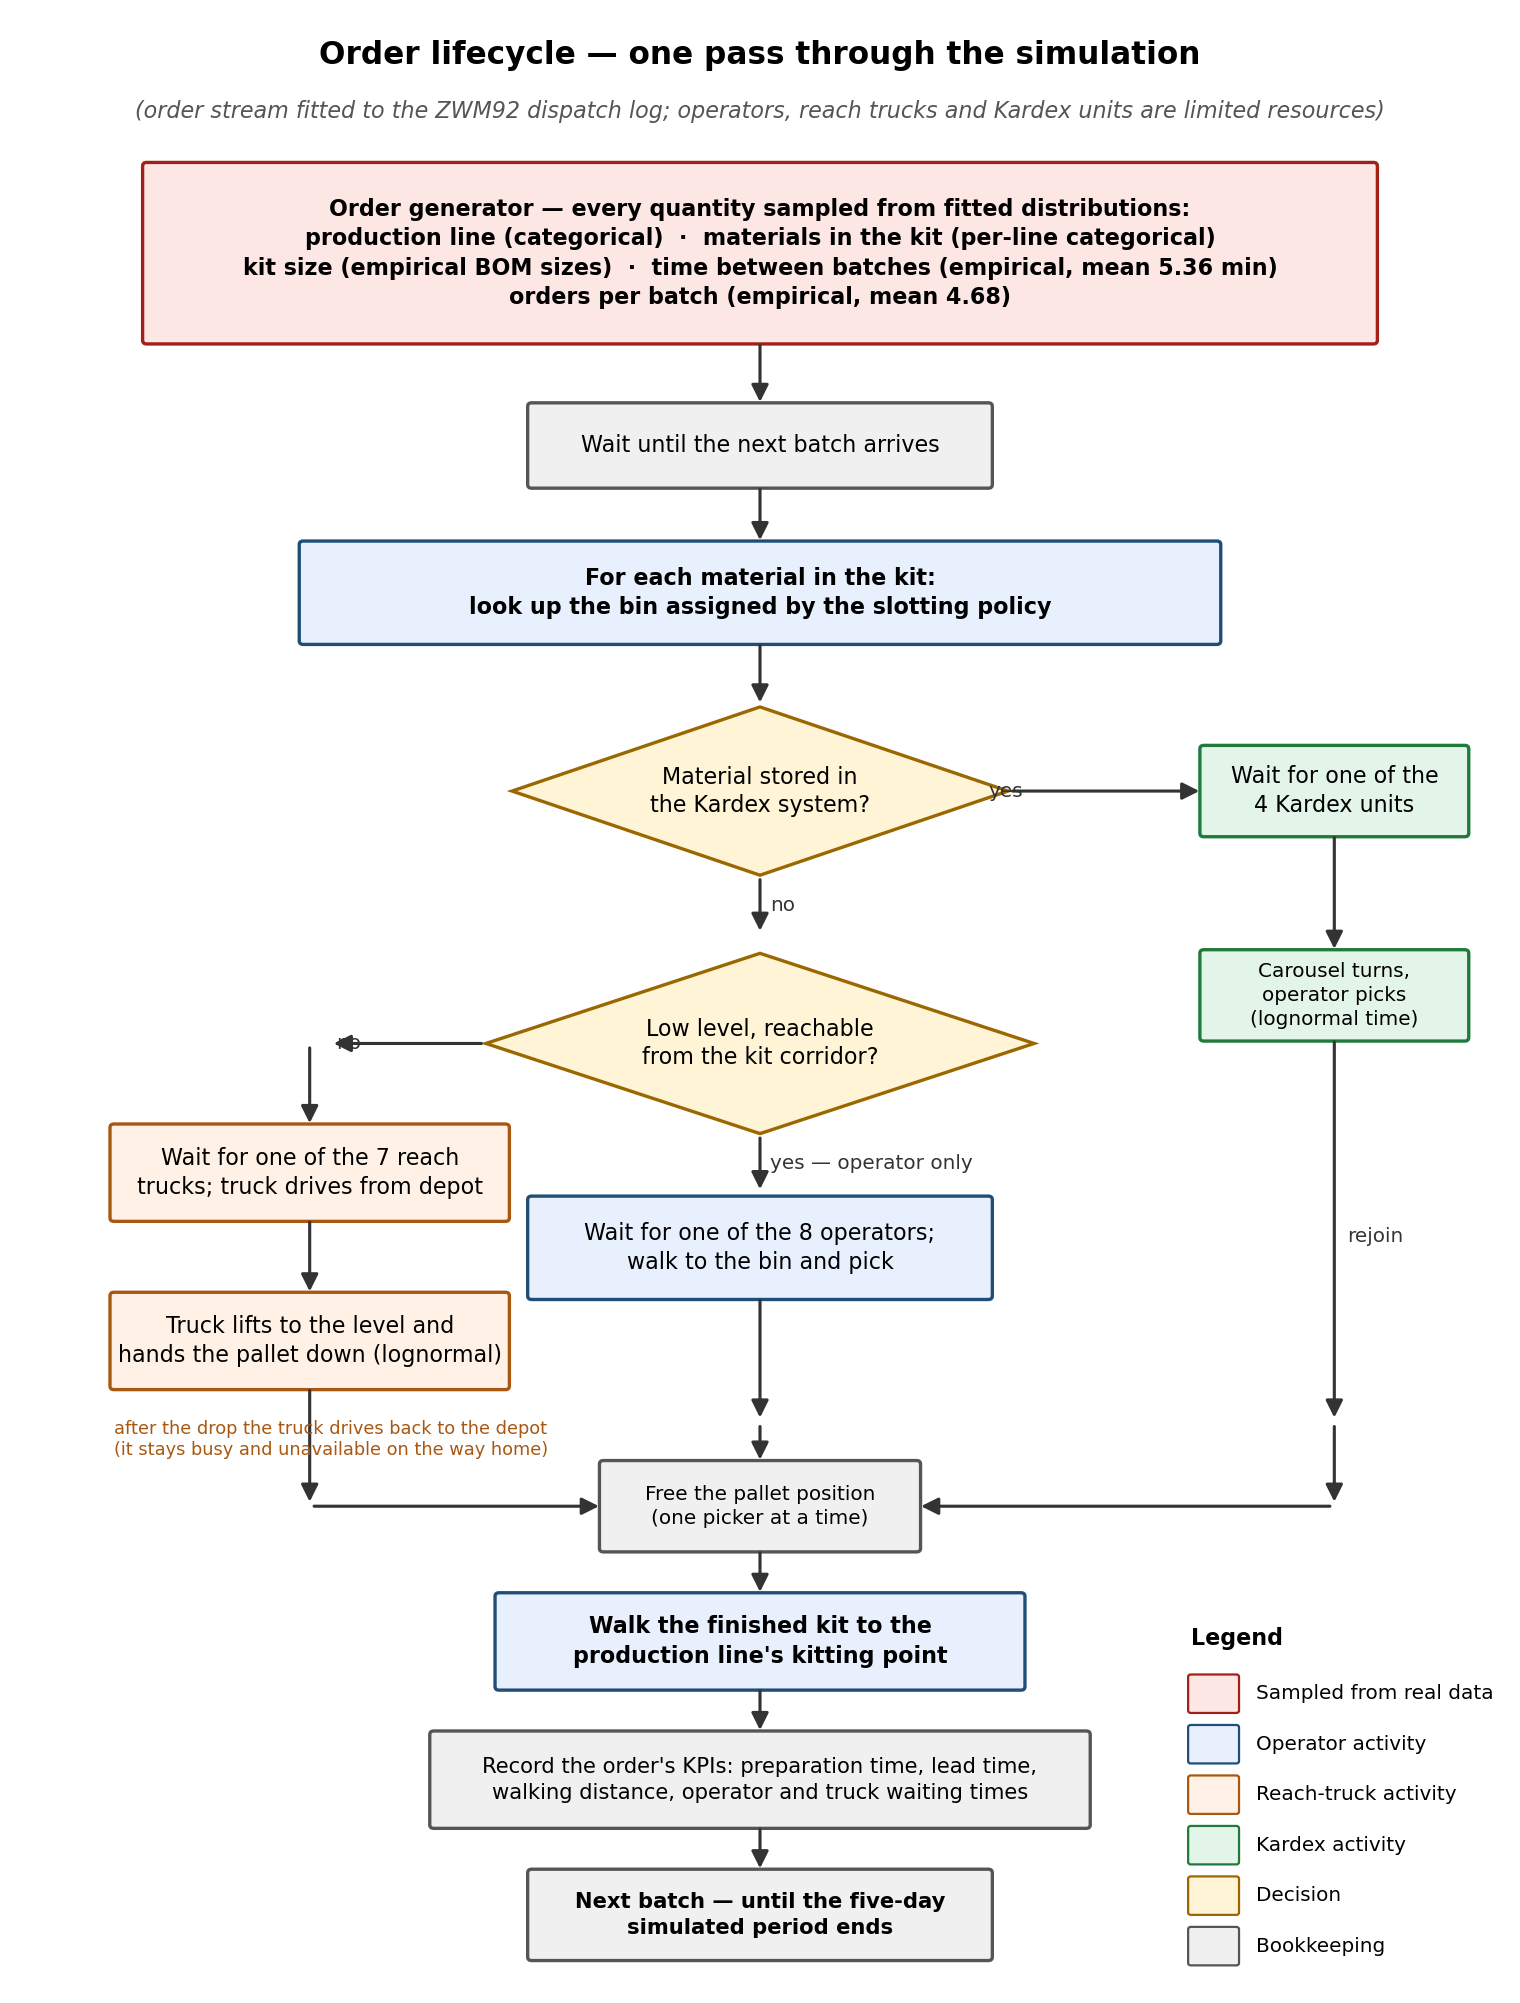
\includegraphics[width=\textwidth]{sim_flowchart_detailed}
  \caption{Detailed simulation flow chart.  The diagram expands
    Figure~\ref{fig:simflow} in the Methodology with all resource-request nodes,
    stochastic-sampling symbols (order inter-batch gap, batch size,
    items per kit, lognormal pick durations), and the reach-truck
    return leg that keeps the RT resource busy until the truck is
    back at the depot.}
  \label{fig:flow_detailed}
\end{figure}

% ─────────────────────────────────────────────────────────
\subsection{Full KPI Table}\label{sec:app_kpi_full}

\begin{table}[htbp]
\centering
\caption{Full KPI table, mean over $N=20$ replications.}
\label{tab:kpi_full}
\scriptsize
\setlength{\tabcolsep}{3pt}
\begin{tabular}{l*{6}{c}}
\toprule
KPI & \makecell{Current\\SAP} & \makecell{Capacity\\heuristic} & \makecell{Usage\\ABC} & \makecell{Double\\ABC} & \makecell{Travel-dist.\\opt.} & \makecell{Line-aware\\slotting} \\
\midrule
Lead time (min) & 12.37 & 14.71 & 15.24 & 14.74 & 24.60 & 6.91 \\
Prep time (min) & 3.92 & 4.31 & 4.43 & 4.34 & 5.62 & 2.65 \\
Total wait (min) & 8.45 & 10.40 & 10.82 & 10.40 & 19.03 & 4.26 \\
P95 lead time (min) & 35.9 & 43.0 & 42.9 & 41.9 & 70.6 & 18.8 \\
Walk distance (m) & 89.0 & 106.1 & 108.8 & 104.6 & 96.1 & 92.4 \\
Throughput (orders/day) & 398.5 & 398.4 & 398.4 & 398.4 & 396.2 & 398.6 \\
RT utilization & 0.217 & 0.228 & 0.244 & 0.246 & 0.440 & 0.013 \\
Operator utilization & 0.405 & 0.446 & 0.457 & 0.448 & 0.576 & 0.275 \\
Kardex utilization & 0.079 & 0.079 & 0.079 & 0.078 & 0.078 & 0.079 \\
Orders completed (5 days) & 1943 & 1942 & 1942 & 1942 & 1931 & 1943 \\
\bottomrule
\end{tabular}
\end{table}


Table~\ref{tab:kpi_full} reports the mean of all ten tracked KPIs over
$N = 20$ paired replications for each policy.
Lead time, total waiting time, RT utilization, and throughput are the
primary comparison metrics discussed in the Results section.
The remaining rows --- prep time, P95 lead time, walking distance,
operator utilization, Kardex utilization, and orders completed over the
five-day run --- are included for completeness and to let readers
cross-check the results in Minitab using the per-replication export
(\texttt{kpi\_by\_replication.csv}).

% ─────────────────────────────────────────────────────────
\subsection{Model Assumption Register}\label{sec:app_assumptions}

Table~\ref{tab:assumptions} lists the twelve modelling assumptions that
most affect the headline KPIs, with the evidence basis for each and the
direction of risk if the assumption proves wrong.
A fuller treatment of each item --- including when assumptions were
revised during the project --- is recorded in \texttt{ASSUMPTIONS.md}
in the project repository.

\begin{table}[htbp]
  \centering
  \caption{Key modelling assumptions, their evidence basis, and the
    direction of error if the assumption is violated.}
  \label{tab:assumptions}
  \small
  \setlength{\tabcolsep}{4pt}
  \begin{tabular}{p{4.8cm} p{4.8cm} p{4.8cm}}
    \toprule
    \textbf{Assumption} & \textbf{Basis} & \textbf{Risk if wrong} \\
    \midrule
    One storage bin per material.  SAP records multiple bins for some
    SKUs; the model assigns each material to a single best-fit slot.
    &
    SAP \texttt{özet} sheet decoded 802 rack bins and 2,872 Kardex
    assignments; for multi-bin materials the nearest bin is used.
    &
    Understates real-warehouse flexibility slightly; the SAP baseline's
    advantage could be marginally lower than reported. \\[4pt]

    Fast-mover manual band: the three lowest rack levels (
    up to $\approx 206$ cm) are reachable without a reach truck.
    &
    Site visit (``first three levels reachable by hand''); corroborated
    by F400 video footage and rack PDF level-height stamps.
    &
    If the real threshold is two levels, manual-band placements are
    over-counted and RT utilization is understated across all policies. \\[4pt]

    F400 timing constants extrapolated to all nine product families.
    Operator pick: 0.113 min; RT pick/place: 0.110 min;
    manual-penalty: 0.102 min; Kardex pick: 0.113 min.
    &
    F400 video time-motion study, 2,319 micro-events, 296.6 min of footage
    (source: \texttt{F400 Kit Cansu Nehir.xlsx}).
    &
    Families with different bin heights or heavier parts may have
    different rates; sensitivity analysis bounds the effect at roughly
    $\pm$15\% on lead time. \\[4pt]

    Service times are lognormal with means from the F400 study and
    log-$\sigma$ moment-matched from the measured CVs
    (operator 1.245, RT 1.047, manual-penalty 1.279, Kardex 1.245).
    &
    F400 CVs: operator pooled CV = 1.93 ($n = 900$); RT CV = 1.41
    ($n = 69$).
    &
    Lognormal may underfit very heavy service tails; if the true
    tail is heavier, RT queue lengths are understated under all
    congestion-prone policies. \\[4pt]

    Batch arrivals: empirical inter-batch gaps and batch sizes sampled
    from the timestamped ZWM92 subset (Okken, AKS\_PAK, F400;
    18,164 orders, 3,885 batches).
    &
    ZWM92 dispatch log; mean batch size 4.68, CV 2.04 (rules out
    Exponential); calibrated at 419 orders/day vs.\ actual 396/day
    ($+5.7\%$, within the $\pm 10\%$ acceptance band).
    &
    Batch sizes are extrapolated from three families to all eight lines;
    if other lines have larger batches, the system is slightly
    under-loaded. \\[4pt]

    Corridor-aware rectilinear routing: travel follows rack-edge safe
    lines; a clear Manhattan L-path is returned immediately; rack
    bodies are treated as obstacles.
    &
    Floor plan from AutoCAD DWG; measured corridor widths: kit 200 cm,
    RT aisles 300--320 cm, perimeter aisles 280--429 cm.
    &
    One-way aisle flow and agent-to-agent congestion are not modelled;
    walk distances are slightly underestimated in high-load scenarios. \\[4pt]

    RT return-to-depot leg: after delivering a pallet the reach truck
    drives back to the depot as a detached process that holds the RT
    resource until arrival.
    &
    DWG floor plan for depot location; standard RT operating procedure
    confirmed at site visit.
    &
    If trucks park near the last delivery point rather than returning to
    depot, RT queue-wait is somewhat overstated; the directional error
    favours Line-aware Slotting (lower RT demand). \\[4pt]

    Kardex single carousel rotation per kit: one rotation is charged
    per kit order regardless of how many Kardex picks that order
    contains; picks inside the rotation are sequential.
    &
    H1 code-audit fix (May 2026); operational semantics of vertical
    carousels confirmed with warehouse staff.
    &
    If each pick triggers an independent rotation, Kardex utilization
    is understated by roughly $3\times$ for kits with multiple Kardex
    items. \\[4pt]

    Single-shift model: ZWM92's four-month dispatch log is compressed
    into an independent 480-minute working day (07:00--16:00 profile).
    Warmup and cooldown windows of 30 min each trim edge effects.
    &
    ZWM92 timestamps span a single shift window; multi-shift dispatch
    patterns were not observed in the log.
    &
    If the real plant runs double shifts, steady-state queue lengths
    could be higher; the model cannot replicate end-of-shift catch-up
    dynamics. \\[4pt]

    Capacity-heuristic placement for undecoded materials (approximately
    2,319 rack materials without a decoded SAP bin): assigned to the
    first free slot in the rack with available capacity.
    &
    750 materials have fully decoded SAP bins; 2,872 are Kardex-routed
    (policy-invariant); the remaining positions use the heuristic.
    &
    The SAP baseline is in practice a SAP+heuristic hybrid; pure SAP
    fidelity is 12.6\% of all active materials (750/5\,941).  Disclosed in the Results
    section. \\[4pt]

    Distribution-driven order arrivals (not trace replay): each
    replication draws fresh samples from fitted distributions with a
    replication-specific seed ($42 + \text{rep}$) and independent
    arrival and service RNG streams.
    &
    Arena-style design per advisor guidance; CRN across policies
    enforced by stream separation.
    &
    Training and validation use the same four-month dataset, so
    the chi-square and volume checks are internal-consistency tests,
    not holdout validation.  Supporting evidence comes from F400 timing,
    daily-volume calibration, and face validity checks in the 3D viewer. \\[4pt]

    Model scope is order picking only; putaway and replenishment are
    out of scope (pallet positions do not deplete).
    &
    Scope agreed with the project supervisor; replenishment scheduling
    was not visible in the ZWM92 dispatch log.
    &
    Line-aware Slotting places fast movers at low (no-RT) levels, which
    would require periodic replenishment in practice.  The policy
    comparison is internally fair --- scope is identical for all six
    policies --- but the RT utilization figures cover picking only. \\
    \bottomrule
  \end{tabular}
\end{table}

% ─────────────────────────────────────────────────────────
\subsection{Software and Reproducibility}\label{sec:app_software}

We wrote the simulation in Python~3 using the SimPy discrete-event
library \cite{simpy}.  The model spans 17 source modules in the
\texttt{src/} directory: data loading and SAP bin decoding,
warehouse geometry and routing, slotting policies, SimPy process logic,
KPI recording, statistical analysis, validation, and sensitivity sweeping.

All statistics in this report are recomputed by script from the
per-replication output files.  Running \texttt{src/main.py} executes the six
policies across 20 replications with common random numbers and writes a
tidy CSV (\texttt{kpi\_by\_replication.csv}) where each row is one
policy--replication pair.  We imported that file directly into Minitab
for the ANOVA and paired $t$-tests in the Results section;
\texttt{src/analyze.py} runs the same tests as a cross-check.
The sensitivity sweeps in \texttt{src/sensitivity.py} apply
one-at-a-time perturbations to each timing constant and produce
the tornado charts in Appendix~\ref{sec:app_sensitivity}.

For face validation we built an interactive 3D warehouse viewer in Three.js.
It renders rack geometry from the AutoCAD DWG and the eleven rack PDF
drawings, animates agent trajectories from the simulation recorder output,
and shows the per-policy KPI comparison panel we used in our project
presentations.

% ─────────────────────────────────────────────────────────
\subsection{Additional Sensitivity Charts}\label{sec:app_sensitivity}

Figure~\ref{fig:sensitivity_2x2} gives OAT tornado charts for three
additional KPIs --- average walking distance, orders completed, and RT
utilization --- alongside the pick-density heatmap for the Usage-based ABC
policy.  The lead-time tornado chart appears in the main Results section.

\begin{figure}[htbp]
  \centering
  \begin{tabular}{cc}
    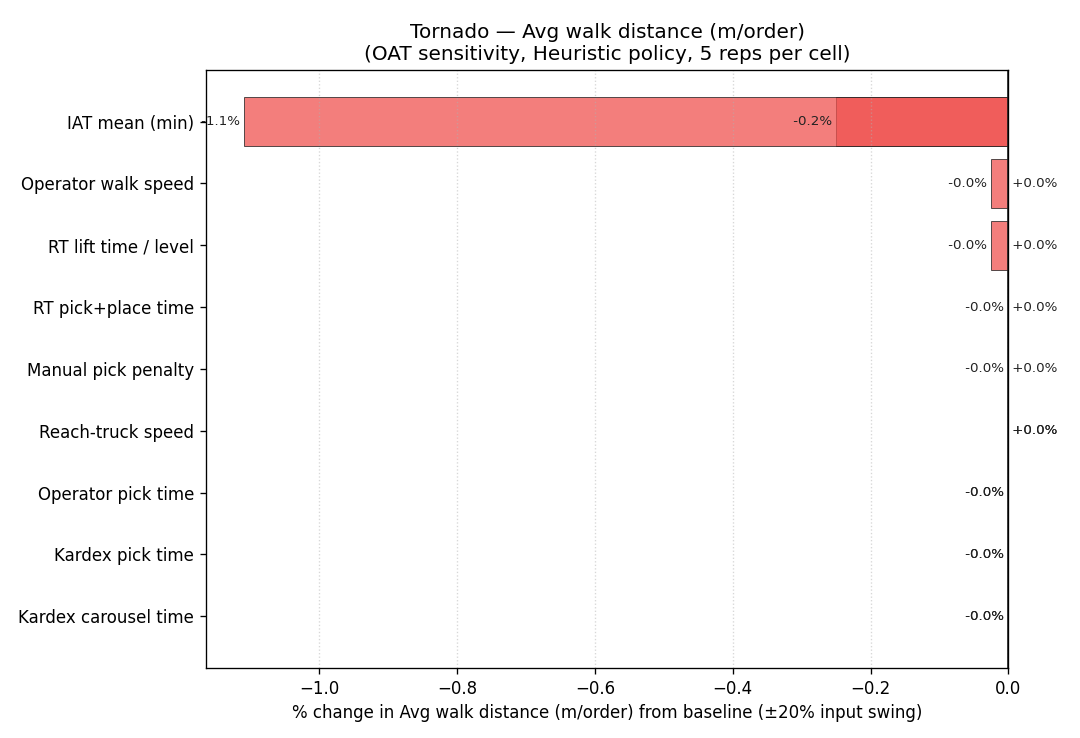
\includegraphics[width=0.47\textwidth]{sensitivity_tornado_avg_walk_distance} &
    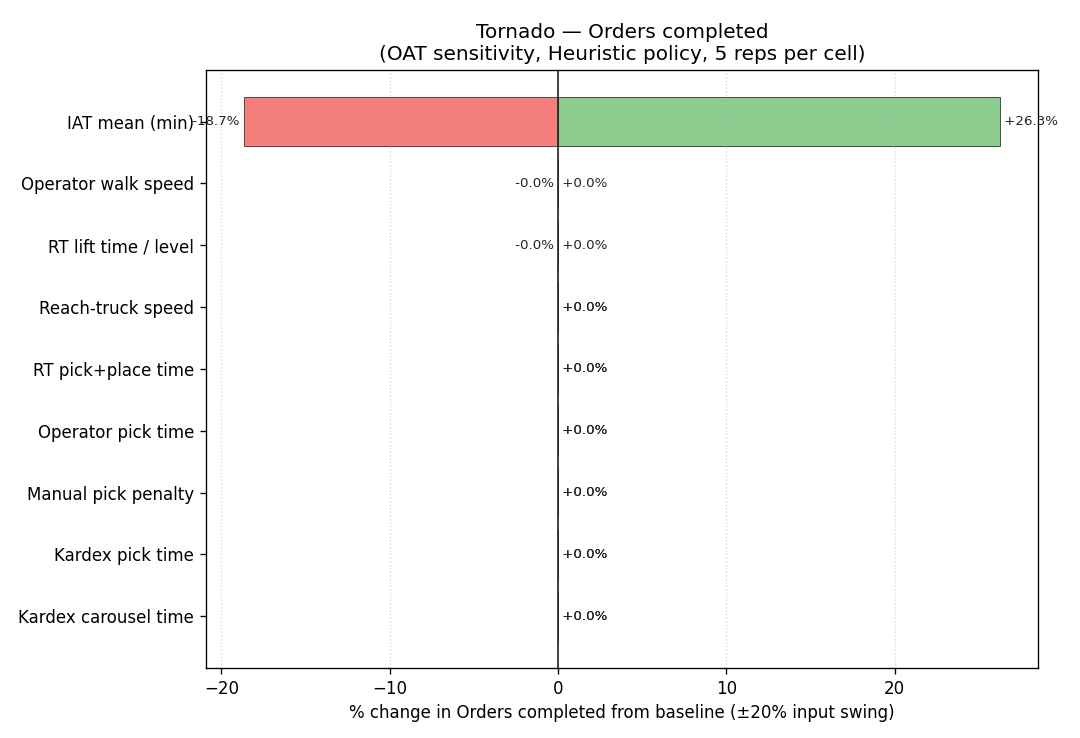
\includegraphics[width=0.47\textwidth]{sensitivity_tornado_orders_completed} \\[6pt]
    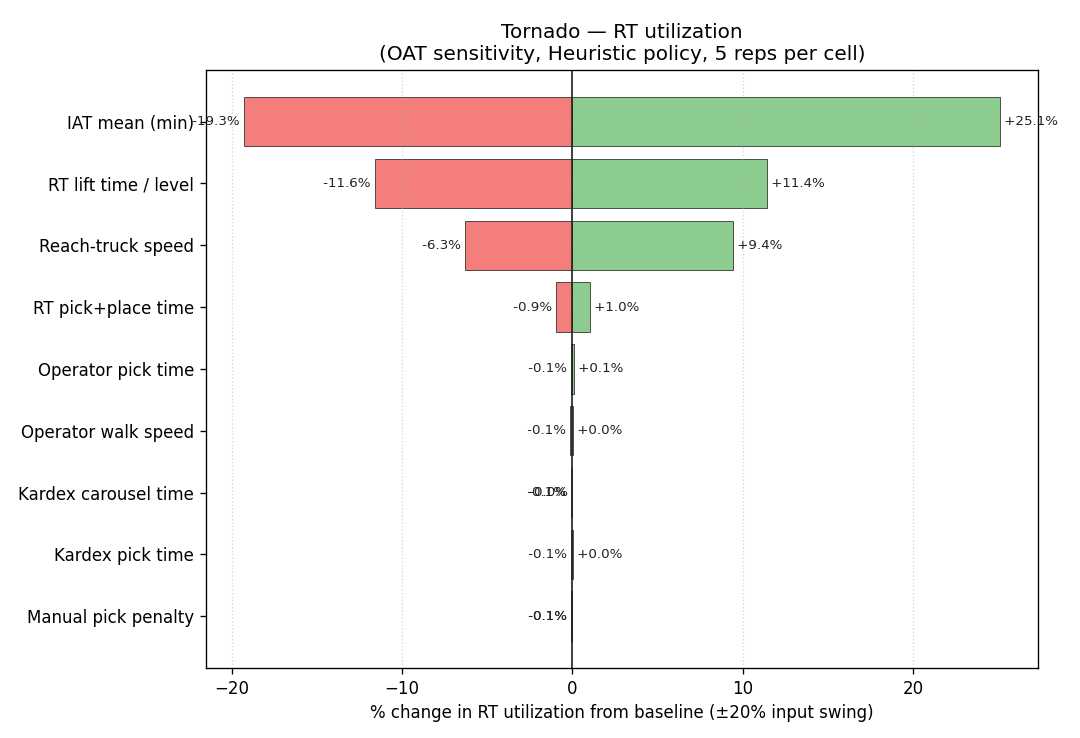
\includegraphics[width=0.47\textwidth]{sensitivity_tornado_reach_truck_utilization} &
    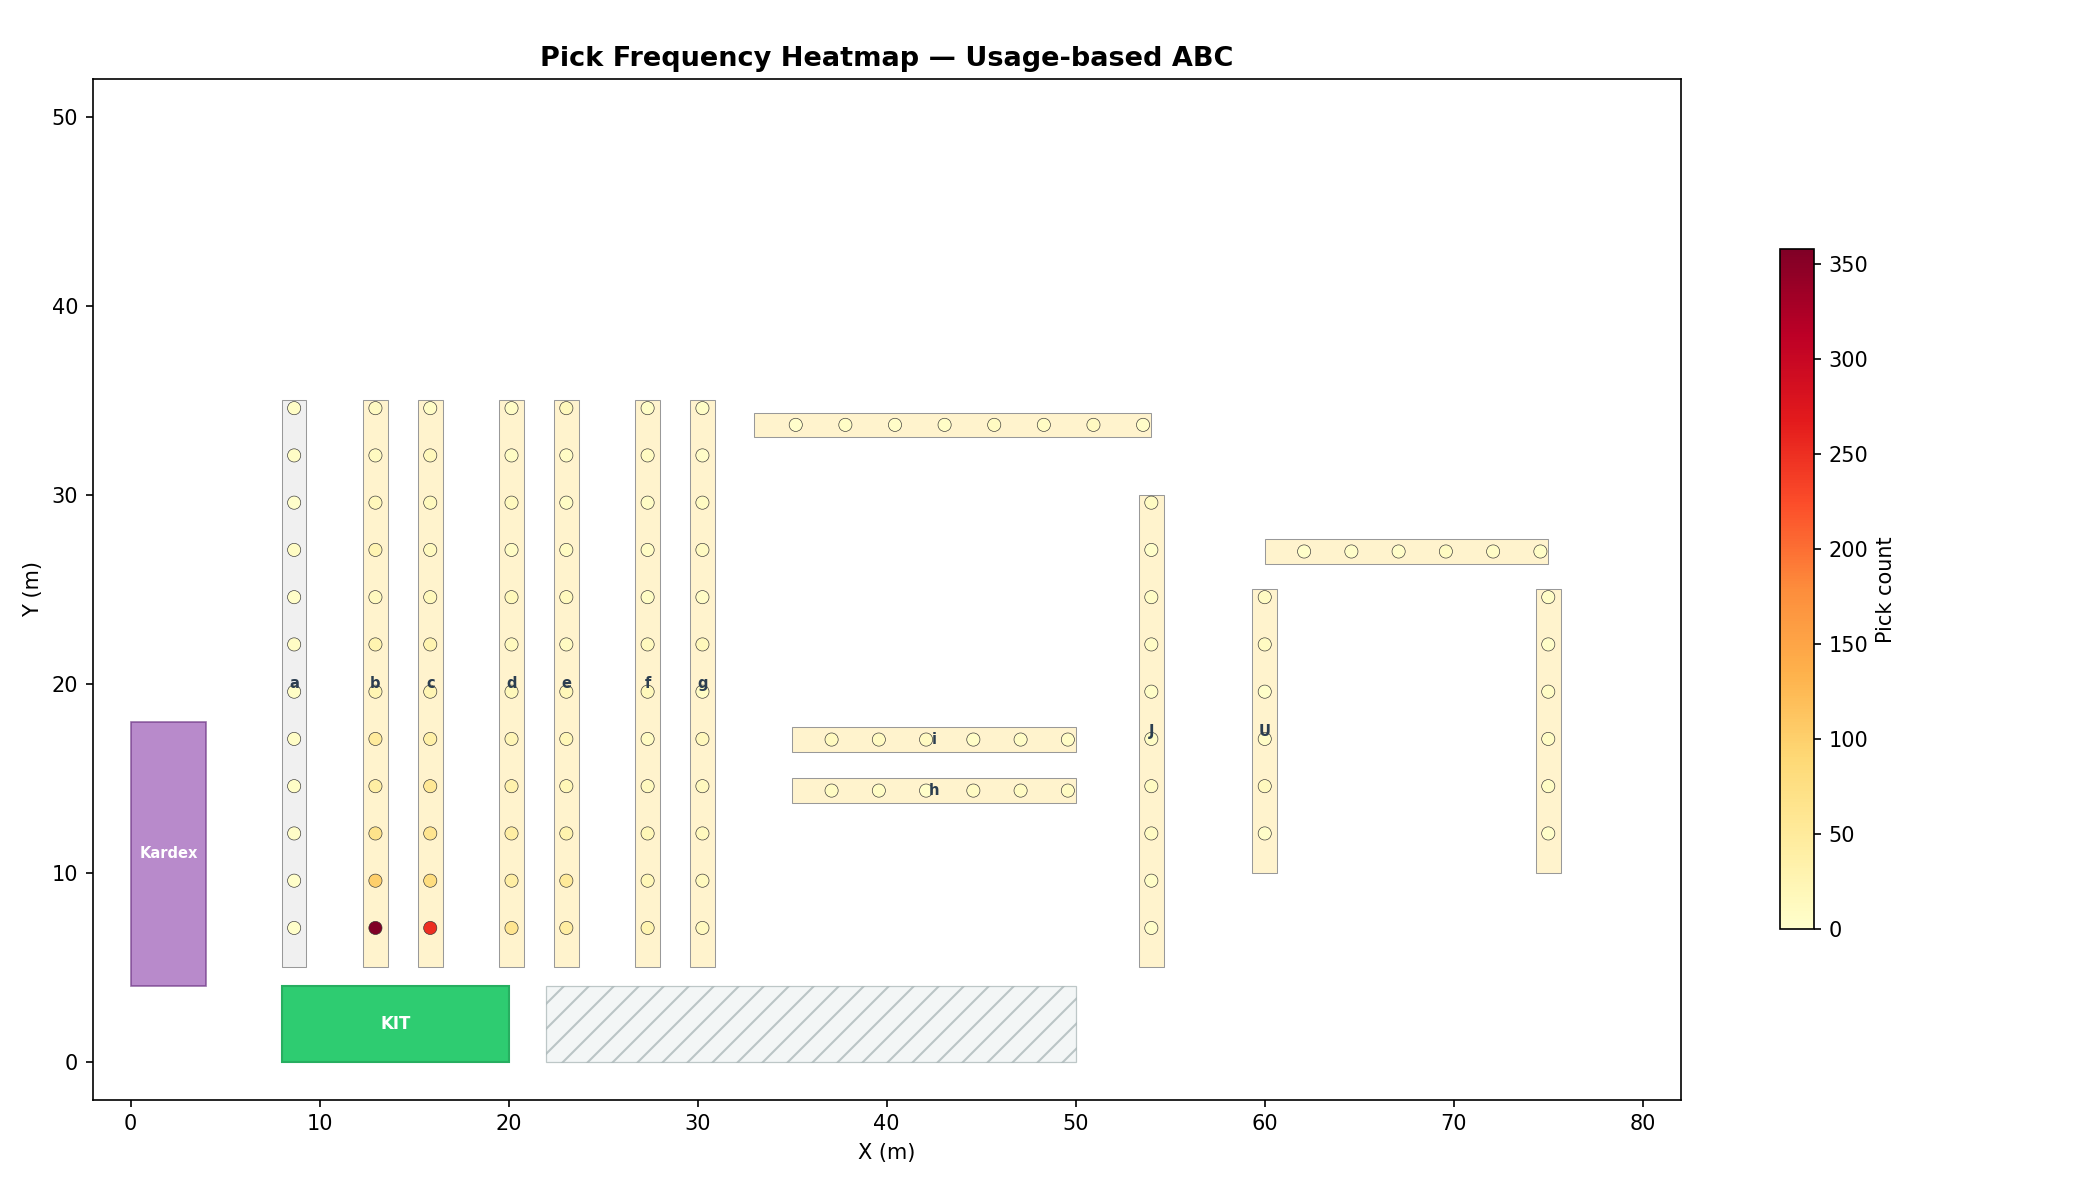
\includegraphics[width=0.47\textwidth]{heatmap_usage-based_abc} \\
  \end{tabular}
  \caption{Top row: OAT tornado charts for average walking distance per
    order (left) and orders completed over the five-day run (right).
    Bottom left: OAT tornado chart for reach-truck utilization, showing
    that the arrival rate and RT lift time are the dominant
    drivers of RT queue load.
    Bottom right: pick-density heatmap for the Usage-based ABC policy,
    showing how that policy distributes frequent picks across the rack
    array; the concentration in the central racks contrasts with the
    line-corridor grouping achieved by Line-aware Slotting.}
  \label{fig:sensitivity_2x2}
\end{figure}


\end{document}
